%%%%%%%%%%%%%%%%%%%%%%%%%%%%%%%%%%%%%%%%
% datoteka diploma.tex
%
% vzorčna datoteka za pisanje diplomskega dela v formatu LaTeX
% na UL Fakulteti za matematiko in fiziko
%
% vkup spravil Gašper Fijavž, december 2010 množica popravkov v januarju,
% februarju marcu 2011 verzijo 29. marec 2011 za FMF 19.9.2013 prilagodil Rok
% Mihevc
%%%%%%%%%%%%%%%%%%%%%%%%%%%%%%%%%%%%%%%%

\documentclass[a4paper, oneside, 12pt]{book}

\usepackage[utf8]{inputenc}
\usepackage[slovene,english]{babel}    % naloži, med drugim,
\usepackage[pdftex]{graphicx}  % omogoča vlaganje slik
\usepackage{fancyhdr}          % poskrbi, na primer, za
\usepackage{amssymb}           % dodatni simboli
\usepackage{amsmath}           % eqref, npr.
\usepackage{verbatim}
\usepackage{float}
\usepackage{tikz}

\renewcommand{\baselinestretch}{1.3} % ustrezen razmik med vrsticami

%oznake strani

\renewcommand{\chaptermark}[1]%
{\markboth{\MakeUppercase{\thechapter.\ #1}}{}} \renewcommand{\sectionmark}[1]
{\markright{\MakeUppercase{\thesection.\ #1}}} \renewcommand{\headrulewidth}{0.5pt} \renewcommand{\footrulewidth}{0pt} 
\fancyhf{}
\fancyhead[LE,RO]{\sl \thepage} \fancyhead[LO]{\sl \rightmark} \fancyhead[RE]{\sl \leftmark}

\newcommand{\BibTeX}{{\sc Bib}\TeX}

\newcommand{\autfont}{\Large} \newcommand{\titfont}{\LARGE\bf}
\newcommand{\clearemptydoublepage}{\newpage{\pagestyle{empty}\cleardoublepage}}
\setcounter{tocdepth}{1}	      % globina kazala

% konstrukti
\newtheorem{izrek}{Izrek}[chapter] \newtheorem{trditev}{Trditev}[izrek]
\newenvironment{dokaz}{\emph{Dokaz.}\ }{\hspace{\fill}{$\Box$}}

\begin{document}
\selectlanguage{slovene}
\frontmatter
\setcounter{page}{1}
\renewcommand{\thepage}{}

\thispagestyle{empty}
\begin{center}
  {\large\sc Univerza v Ljubljani\\
    Fakulteta za Matematiko in Fiziko\\
    Oddelek za Fiziko\\
  Univerzitetni študij, naravoslovna smer}
  \vskip 10em
  {\autfont Rok Mihevc \par}
  {\titfont Kraške vrtače Dinarskega krasa \par}
  {\vskip 2em \textsc{DIPLOMSKO DELO}\par}
  \vfill
  \null
  {\large \textsc{Mentor}: prof.\ dr.  Rudolf Podgornik\par}
    %  {\large \textsc{Somentor}:  izr.\ prof.\ dr. \par}%
  {\vskip 2em \large Ljubljana, 2014 \par}
\end{center}

\clearemptydoublepage \clearemptydoublepage

\vspace*{1cm}
\begin{center} {\Large \textbf{\sc Izjava o avtorstvu diplomskega dela}} \end{center}

  \vspace{1cm} \noindent Spodaj podpisani Rok Mihevc, z vpisno številko
  \textbf{28030017}, sem avtor  diplomskega dela z naslovom:

  \vspace{0.5cm} \emph{Kraške vrtače Dinarskega krasa}

  \vspace{1.5cm} \noindent S svojim podpisom zagotavljam, da: \begin{itemize}
    \item sem diplomsko delo izdelal samostojno pod mentorstvom prof.\ dr.\
      \mbox{Rudolfa} \mbox{Podgornika}, %in somentorstvom izr.\ prof.\ dr.\,

    \item	so elektronska oblika diplomskega dela, naslov (slov., angl.), povzetek
      (slov., angl.) ter ključne besede (slov., angl.) identični s tiskano obliko
      diplomskega dela \end{itemize}

      \vspace{1cm} \noindent V Ljubljani, dne . februarja 2014 \hfill Podpis avtorja:

    % prazna stran
      \clearemptydoublepage

      \begin{comment}
    %%%%%%%%%%%%%%%%%%%%%%%%%%%%%%%%%%%%%%%%
    % zahvala
      \thispagestyle{empty}\mbox{}\vfill\null\it% Staršema za podporo. \rm\normalfont

    % prazna stran
      \clearemptydoublepage

    %%%%%%%%%%%%%%%%%%%%%%%%%%%%%%%%%%%%%%%%
    % posvetilo
      \thispagestyle{empty}\mbox{}{\vskip0.20\textheight}\mbox{}\hfill\begin{minipage}{0.55\textwidth}%
        Svoji dragi Alenčici. \normalfont\end{minipage}

    % prazna stran
        \clearemptydoublepage

    %%%%%%%%%%%%%%%%%%%%%%%%%%%%%%%%%%%%%%%%
    % ODREZANA NASLOVNICA ITD. DO KAZALA
        \end{comment}

  % kazalo
        \def\thepage{}% preprecimo tezave s stevilkami strani v kazalu
        \tableofcontents{}

  % prazna stran
        \clearemptydoublepage

    %%%%%%%%%%%%%%%%%%%%%%%%%%%%%%%%%%%%%%%%
    % povzetek 
        \addcontentsline{toc}{chapter}{Povzetek} 
        \chapter*{Povzetek}

        Z numeričnimi metodami obdelamo $60 km^2$ velik digitalni model reliefa Menišije ločljivosti $1m^2$ in identificiramo veliko število kraških vrtač. Iz oblik velikega števila vrtač izračunamo povprečno obliko vrtače in jo analitično opišemo z gaussovo funkcijo. Odkrite realne vrtače nato prilegamo na gaussovo funkcijo ter pogledamo porazdelitev parametrov le-te na našem vzorcu.

        Zaradi geološke zgodovine področja Menišije in medsebojne podobnosti vrtač na tem območju postavimo tezo, da jih je oblikoval isti geomorfološki proces, ki vodi do vsem skupne stabilne oblike, ki so jo vrtače na tem območju že dosegle.
        S pomočjo podatkov pridobljenih v prvem delu naloge predlagamo časovno statičen nastavek, ki analitično opiše najdene vrtače. Postavimo tezo, da vrtače oblikuje stohastično priraščanje površja, ter primerjamo teoretično pričakovan eksponent hrapavosti z izmerjenim. Pogledamo še nekaj determinističnih difuzijsko-reakcijskih sistemov, ki bi lahko služili kot dinamični model nastanka vrtač.


        \clearemptydoublepage

    %%%%%%%%%%%%%%%%%%%%%%%%%%%%%%%%%%%%%%%%
    % abstract
        \selectlanguage{english} \addcontentsline{toc}{chapter}{Abstract}
        \chapter*{Abstract}
        Abstract

        \selectlanguage{slovene}
    % prazna stran
        \clearemptydoublepage

        \mainmatter
        \setcounter{page}{1}
        \pagestyle{fancy}

        \chapter{Uvod}
        \label{uvod}

        \begin{figure}[H]
          \begin{center}
            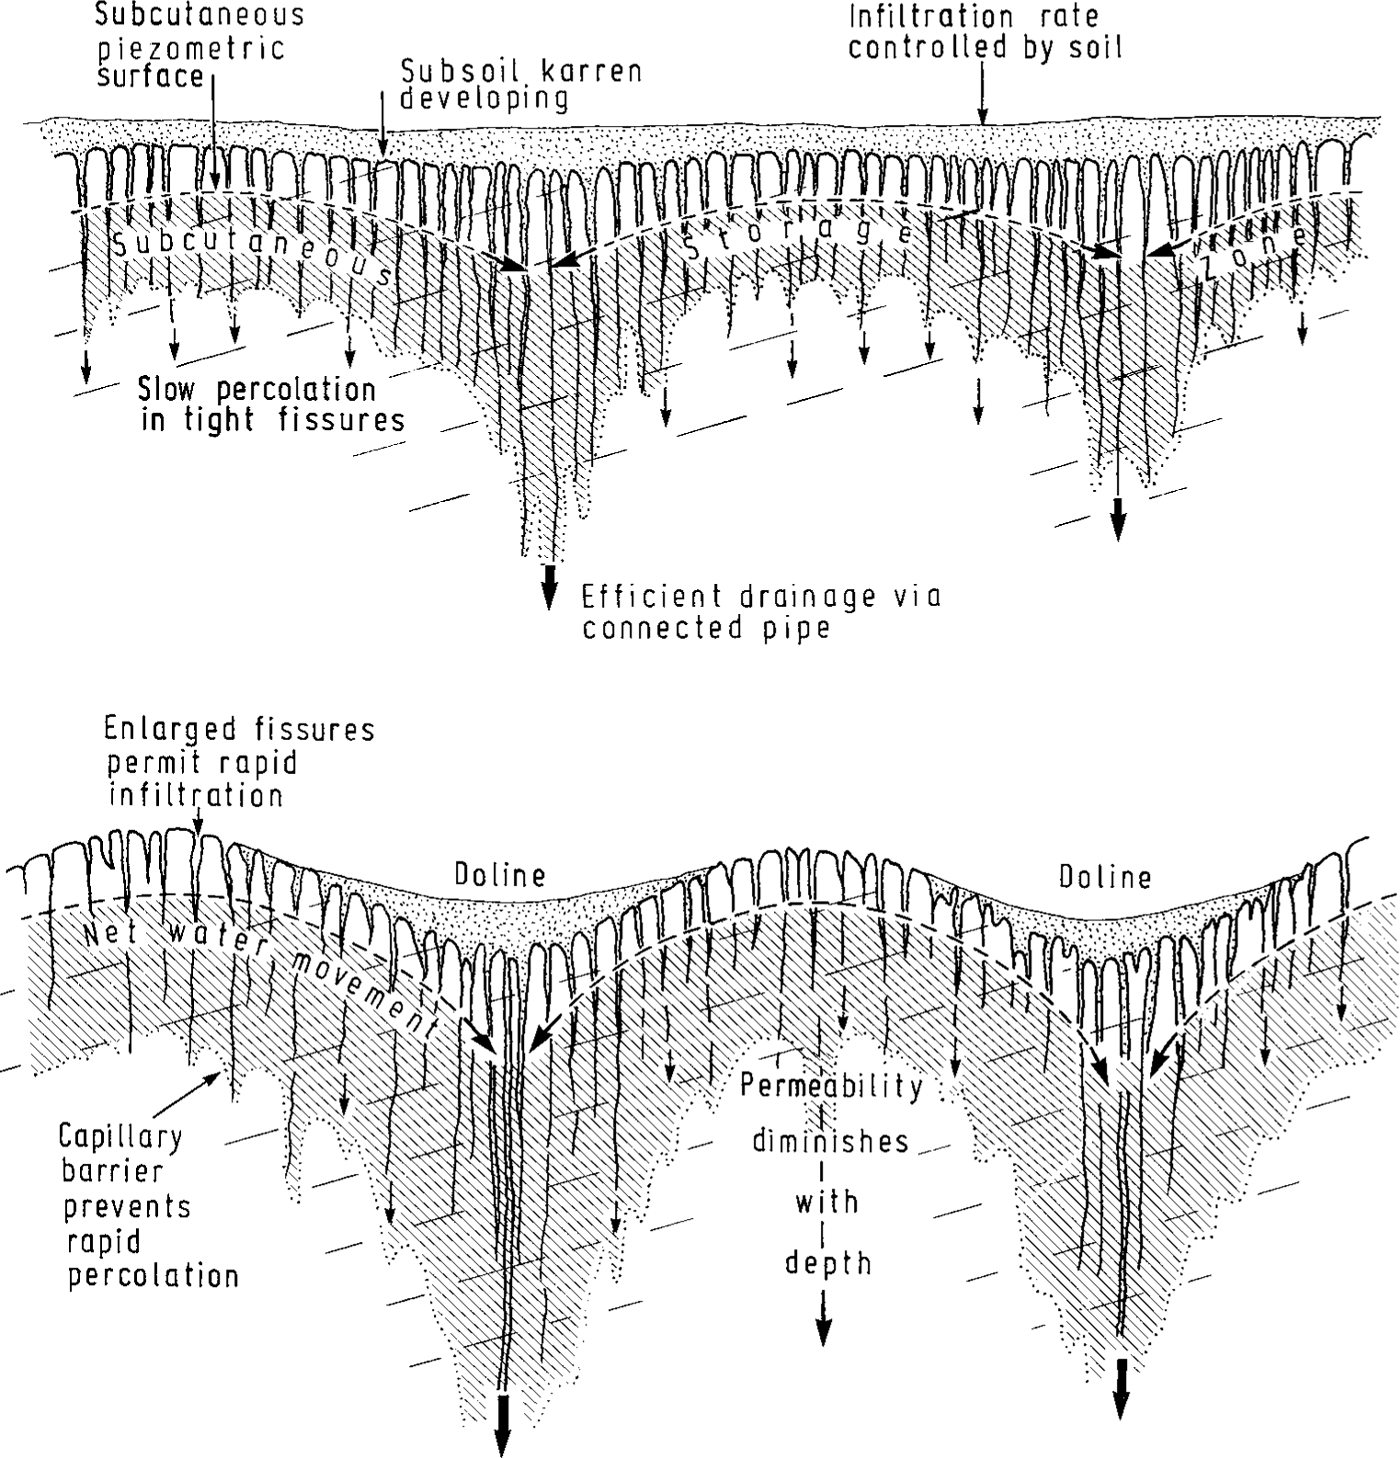
\includegraphics[width=10cm]{slike/vrtaca-ford-williams}
          \end{center}
          \caption{Priljubljena geomorfološka shema za razlago vrtač. Vir: \cite{ford2007karst}}
          \label{fig:vrtaca-ford-williams}
        \end{figure}

        Namen tega dela je na podlagi digitalnega modela reliefa dokumentirati in statistično preučiti velik vzorec realnih kraških vrtač na slovenskem Dinarskem krasu, predlagati analitično funkcijo, ki bi opisala idealno vrtačo, ter na podlagi le-te poiskusiti modelirati naravne procese, ki povzročajo nastanek in obliko vrtač.

        Vrtače so zaobljene lijakaste globeli, globine nekaj metrov in premera nekaj deset metrov. Obstaja več geomorfoloških modelov njihovega nastanka.

        Za študij realnih vrtač uporabimo digitalni model reliefa Menišije (Slika \ref{fig:menisija-karta}) ločljivosti 1m, ki omogoča zanesljivo identifikacijo in študij vrtač ter udornic (Slika \ref{fig:menisija-relief}).

        \begin{figure}[H]
          \centering
          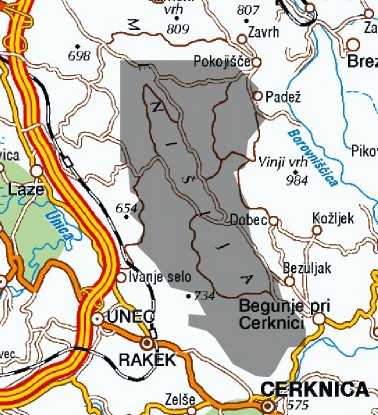
\includegraphics[width=8cm]{slike/menisija-karta}
          \caption{Menišija, $60 km^2$ veliko območje med Cerknico in Logatcem, vsebuje nekaj tisoč vrtač in več udornic in predstavlja približno odstotek slovenskega krasa. Vir: Geopedia, Geodetski inštitut Slovenije}
          \label{fig:menisija-karta}
        \end{figure}

        Površje Menišije sestavljajo plasti krednega apnenca (starost nastanka 135-65 miljonov let), ki so na površje prišli zaradi dogodkov povezanih s podrivanjem Adriatske plošče (17-7 miljonov let). Menišija je bila uravnano kraško polje do 3.5 miljona let pred sedanjostjo, ko se je zaradi tektonske aktivnosti dvignila nad okolico in vzpostavljeni so bili hidrološki pogoji za nastanek vrtač. Hitrost zniževanja (denudacije) kraškega površja se ocenjuje na 20-50 m / miljon let, torej se je površje Menišije v času od nastanka znižalo za 70-175m, hkrati pa so se v njem pojavile vrtače, udornice in brezstrope jame. \cite{Vrabec2006} \cite{Placer2010}

        \begin{figure}[H]
          \begin{center}
            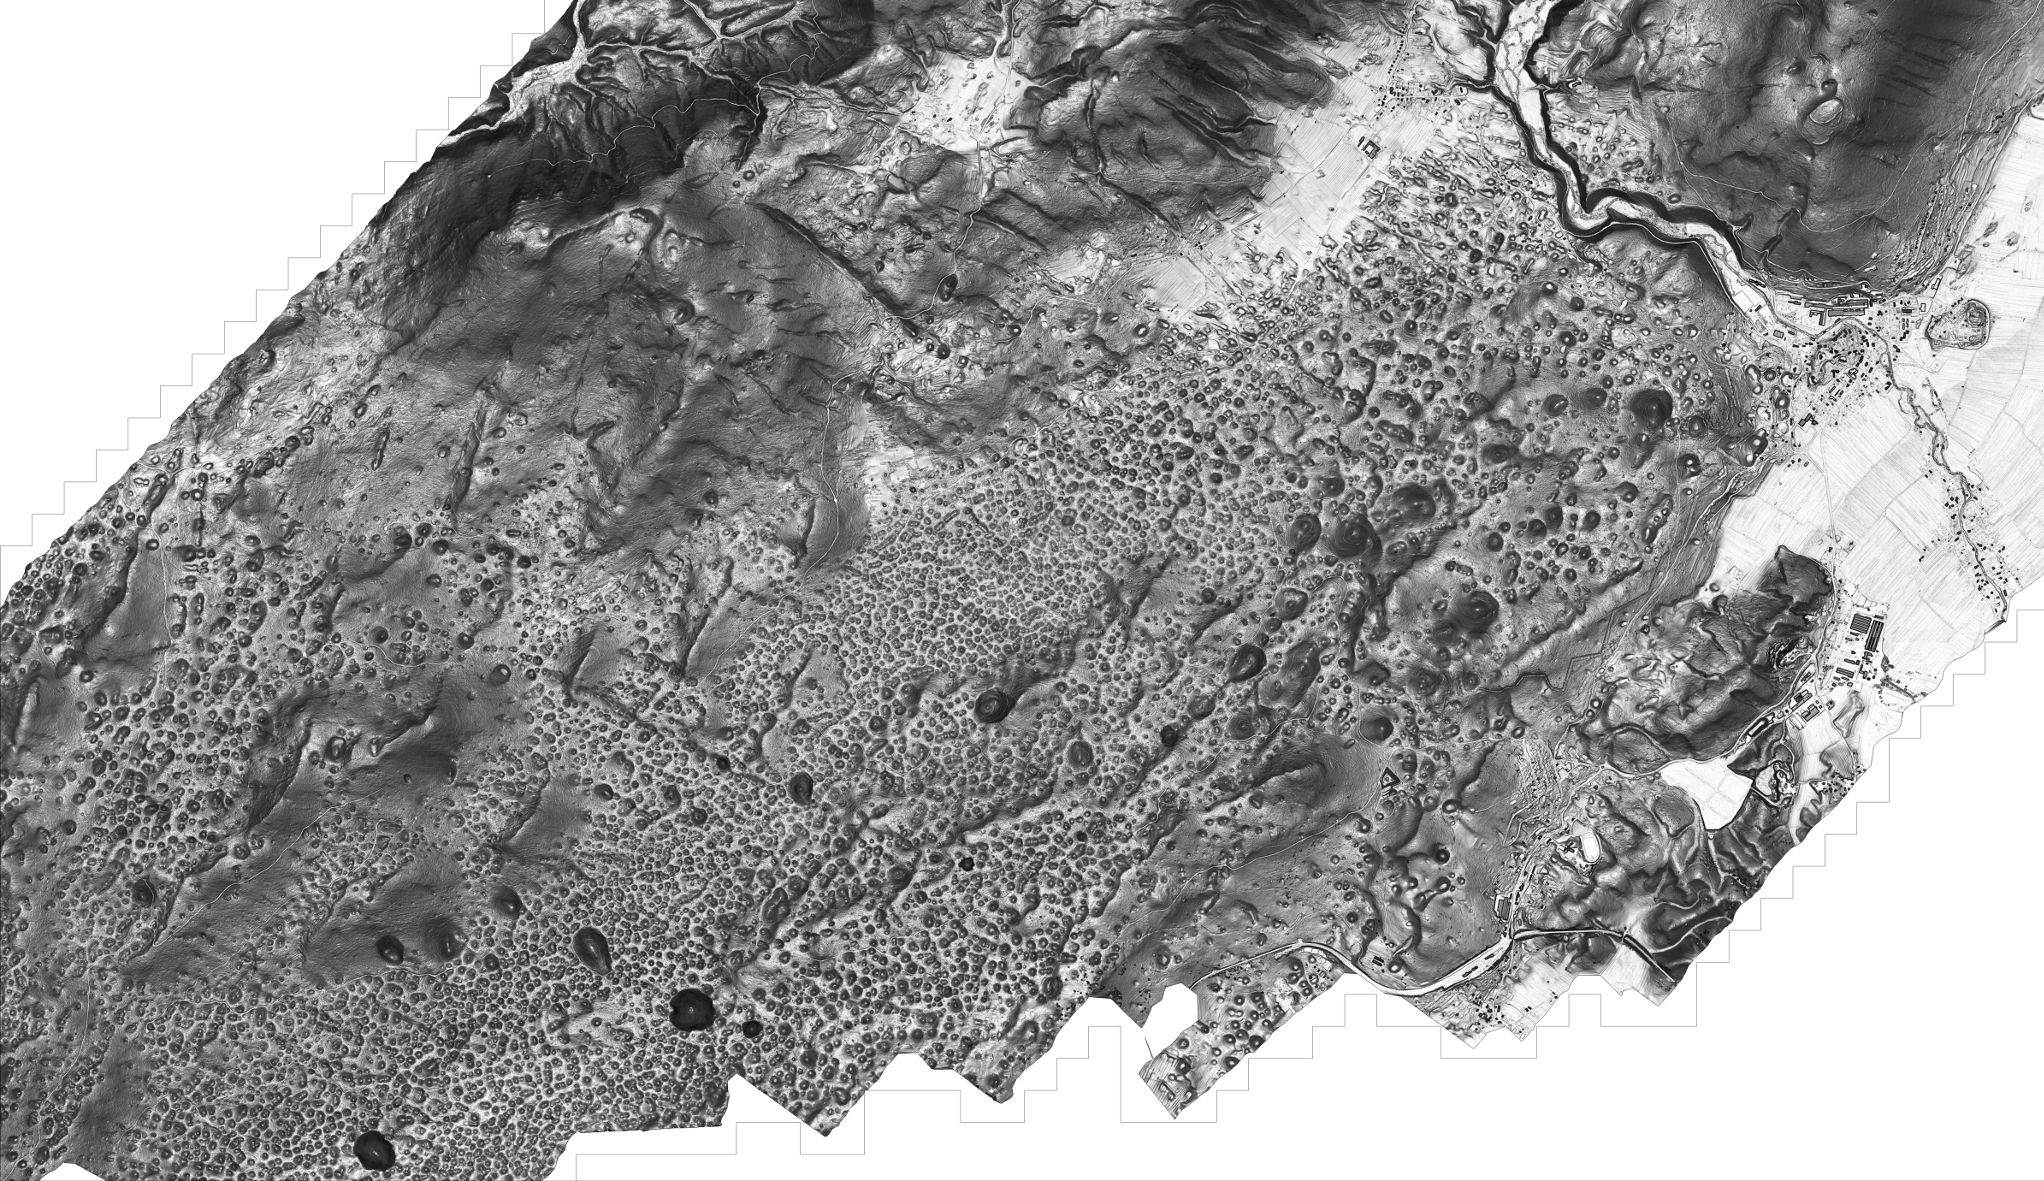
\includegraphics[width=12cm]{slike/menisija-relief}
          \end{center}
          \caption{Senčen 3D relief dela Menišije uporabljen v tej nalogi. Vir: Geodetski inštitur Slovenije \cite{LAK} po metodi \cite{Kobler20079}.}
          \label{fig:menisija-relief}
        \end{figure}

        \chapter{Preučevanje realnih vrtač}
        \label{realne-vrtace}
        Identifikacijo velike količine objektov se lotimo s segmentacijo po konkavnosti, kot predlaga \cite{doctor13}. Točke, ki so nižje od svoje okolice, imajo nižji indeks konkavnosti, točke višje od svoje okolice pa višjega. Pri tem je pomembna tudi pametna izbiro okolice - od nje je odvisno kako velike konkavnosti bomo zaznali. Končno zavržemo konveksne dele površja in konkavne odberemo kot vrtače. Rezultat vidimo na (Slika \ref{fig:menisija-vrtace}). Opaziti velja, da izbrana metoda segmetacije del robov konkavnih objektov klasificira kot konveksne in zato podceni radij. Za naše namene to ni pretirano moteče, saj to podcenitev zlahka kompenziramo kasneje.

        \begin{figure}[H]
          \begin{center}
            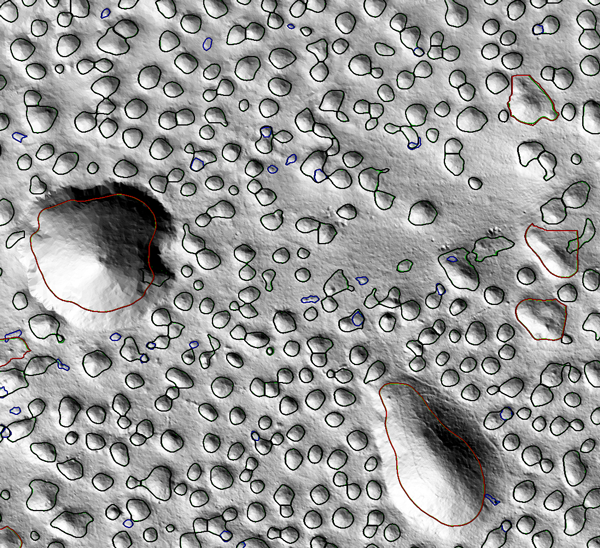
\includegraphics[width=13cm]{slike/menisija-vrtace}
          \end{center}
          \caption{Del od 8687 zaznanih konkavnih objektov na območju Menišije. Poleg vrtač so na sliki vidne tudi udornice.}
          \label{fig:menisija-vrtace}
        \end{figure}

        Najdeni konkavni objekti imajo porazdelitev efektivnih polmerov (\mbox{$r_{eff}=\sqrt{\frac{A_{eff}}{\pi}}$}), kot vidno na (Slika \ref{fig:menisija-polmeri-hist}).

        \begin{figure}[H]
          \centering
          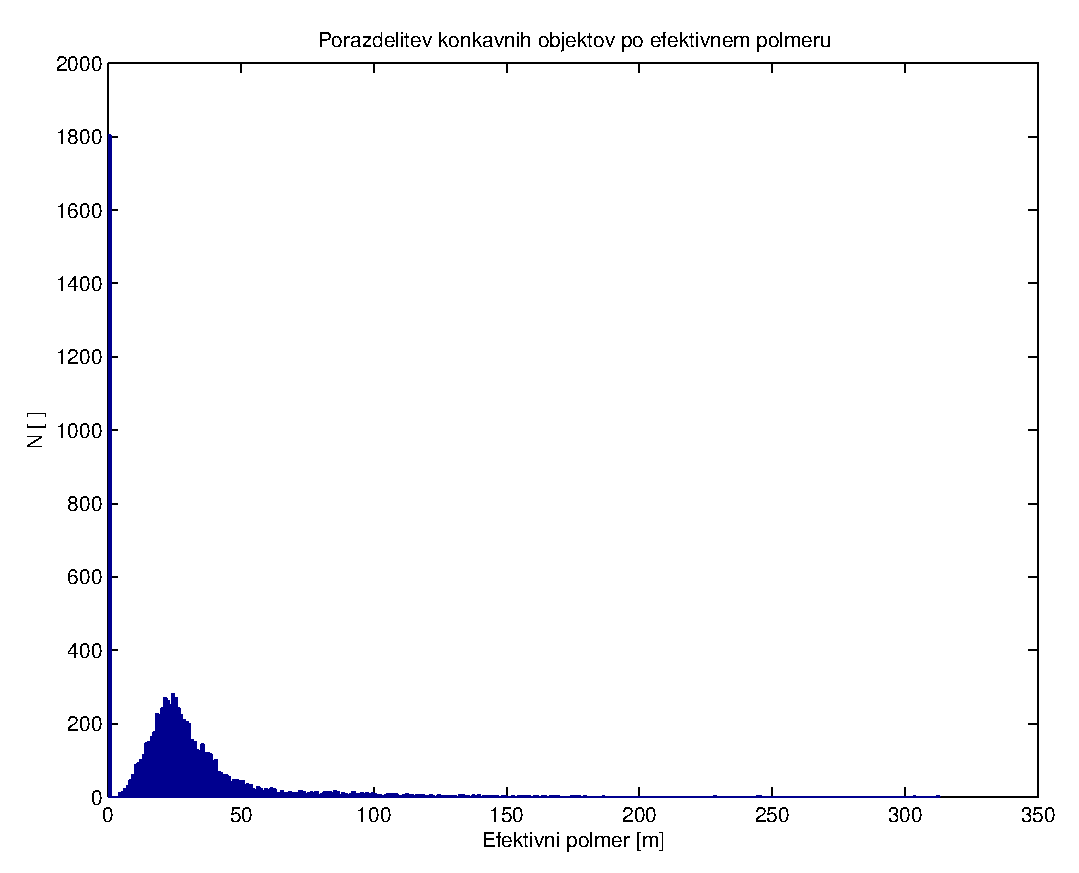
\includegraphics{slike/menisija-polmeri-hist}
          \caption{Polmeri konkavnih objektov v Menišiji, vrh pade v razred od 24m do 25m.}
          \label{fig:menisija-polmeri-hist}
        \end{figure}

        To daje slutiti, da bodisi obstaja ravnovesna velikost vrtače, h kateri konvergirajo vse konkavne oblike v območju ne glede na njihov nastanek, bodisi da so vsi konkavni objekti v tem območju nastali v kratkem časovnem obdobju in se razvijali z enako hitrostjo. Odločimo se za raziskovanje prve možnosti.
        Predvidevamo torej, da obstaja ravnovesna oblika vrtače, ki bi se pojavila na idelani podlagi, če bi preteklo dovolj časa.

        Posamezne realne vrtače zaradi lokalnih pogojev in zgodovine razvoja reliefa niso simetrične, a zdi se, da so si med seboj podobne. Da bi ugotovili idealno obliko vrtače, izračunamo povprečje velikega števila realnih vrtač. Uporabimo dva pristopa - pri prvem (Slika \ref{fig:menisija-vrtaca}) vrtače različnih velikosti raztegnemo in povprečimo, pri drugem (Slika \ref{fig:menisija-vrtace-po-razredih}) pa jih razdelimo v velikostne razrede in jih povprečimo znotraj le-teh. 

        \begin{figure}[H]
          \centering
          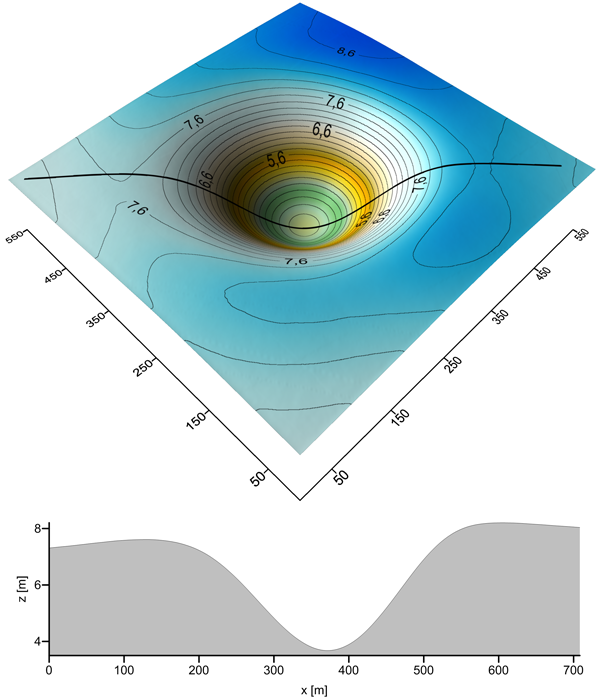
\includegraphics[width=10cm]{slike/menisija-vrtaca}
          \caption{Povprečje 8687 realnih vrtač z območja Menišije, pred povprečjem so bile vrtače raztegnjene na velikost največje v setu.}
          \label{fig:menisija-vrtaca}
        \end{figure}

        \begin{figure}
          \centering
          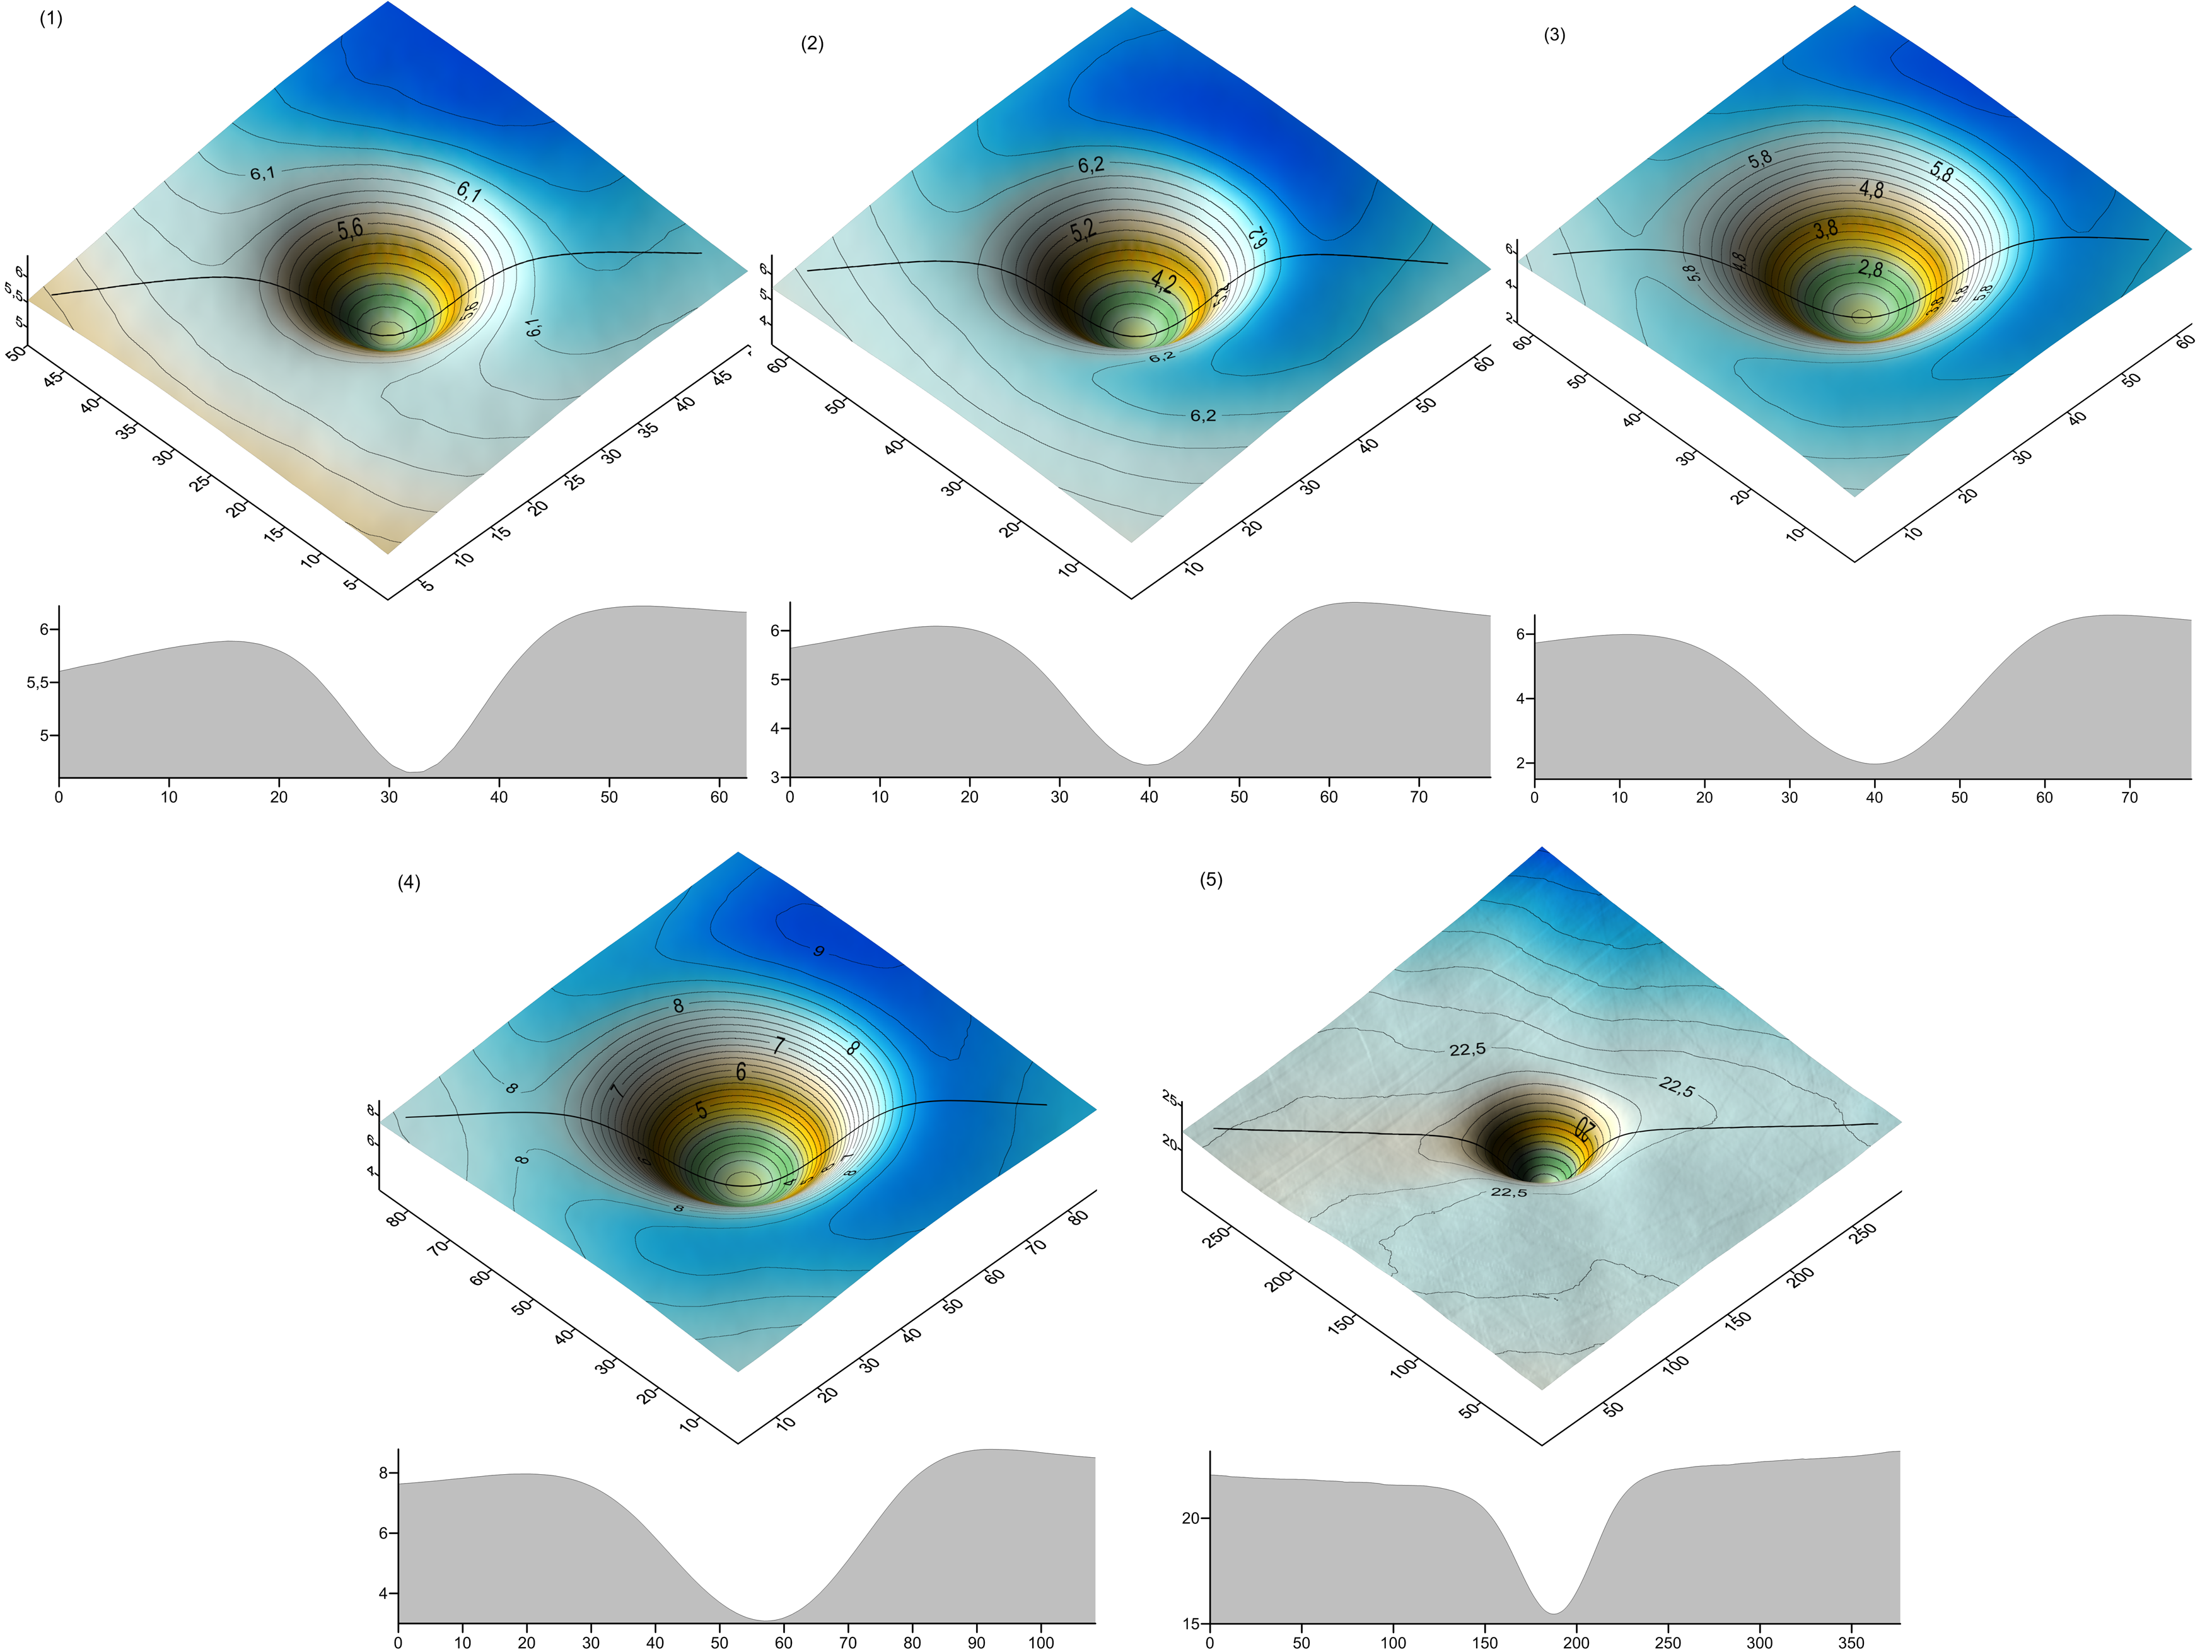
\includegraphics[width=19cm,angle=90]{slike/vrtace-po-razredih-menisija}
          \caption{Vrtače po velikosti razdelimo v pet razredov (najmanjša petina gre v prvi razred, itn.) in jih znotraj razredov povprečimo.}
          \label{fig:menisija-vrtace-po-razredih}
        \end{figure}

        Na prvi pogled se zdijo dobljeni profili gaussove oblike (\ref{fit-vrtace}), kar ne zbuja nujno zaupanja v metodo. Zdi pa se, da so oblike simetrične po kotu, torej lahko problem reduciramo na študij njihovih profilov. 

        \begin{equation}
          f(x,y) = A \cdot e^{-\frac{(x-x_0)^2}{\sigma_x^2}-\frac{(y-y_0)^2}{\sigma_y^2}} + B \cdot x + C \cdot y + D  
          \label{fit-vrtace}
        \end{equation}

        Rezultat uporabimo tako, da gaussovo funkcijo nalegamo na realne vrtače in tako dobimo dobre lokacije njihovih najnižjih točk, ter njihove $\sigma_x$ in $\sigma_y$. Z lokacijami najnižjih točk lahko izračunamo povprečne profile vrtač ($z(r)$), ki imajo enake efektivne polmere, npr. (Slika \ref{fig:menisija-profil-21-fit}).

        \begin{figure}[H]
          \centering
          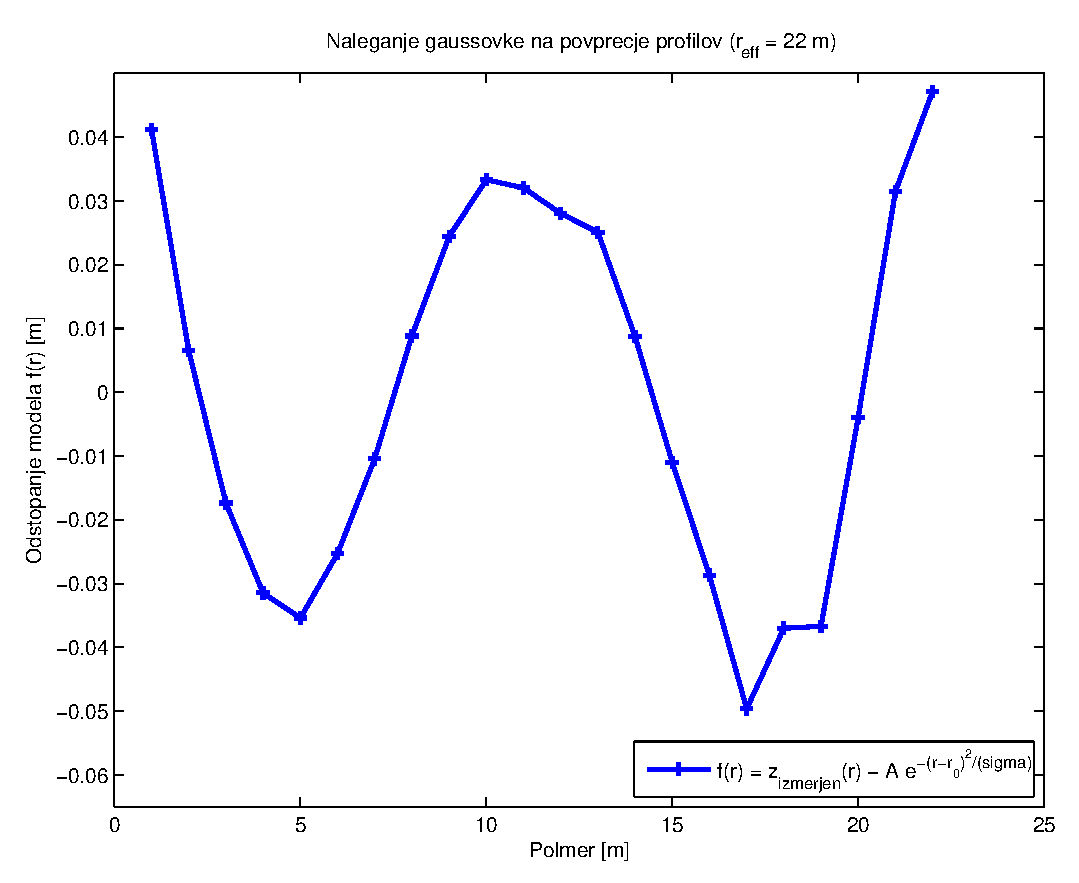
\includegraphics{slike/menisija-profil-21-fit}
          \caption{Povprečje profilov vrtač z efektivnimi polmeri med 23,5m in 24,5m. Prilegamo gaussovko (\ref{fit-profila}). Graf prikazuje razliko med povprečnim profilom in prilegano gausovko.}
          \label{fig:menisija-profil-21-fit}
        \end{figure}

        Pri tem pa je porazdelitev uteži gaussove funkcije (Slika \ref{fig:menisija-globine-hist}), porazdelitev $\sigma$ pa (Slika \ref{fig:menisija-sigme-hist}).

        \begin{figure}[H]
          \begin{center}
            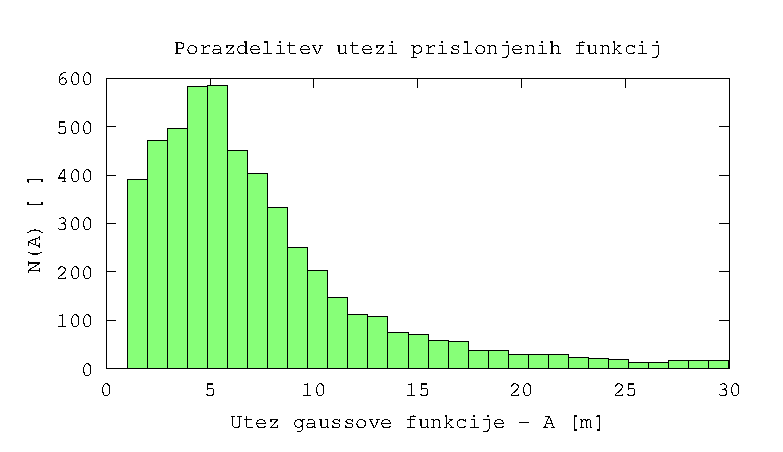
\includegraphics{slike/menisija-globine-hist}
          \end{center}
          \caption{Porazdelitev uteži A za gaussovo funkcijo prilegano na vrtače v Menišiji}
          \label{fig:menisija-globine-hist}
        \end{figure}

        \begin{figure}[H]
          \begin{center}
            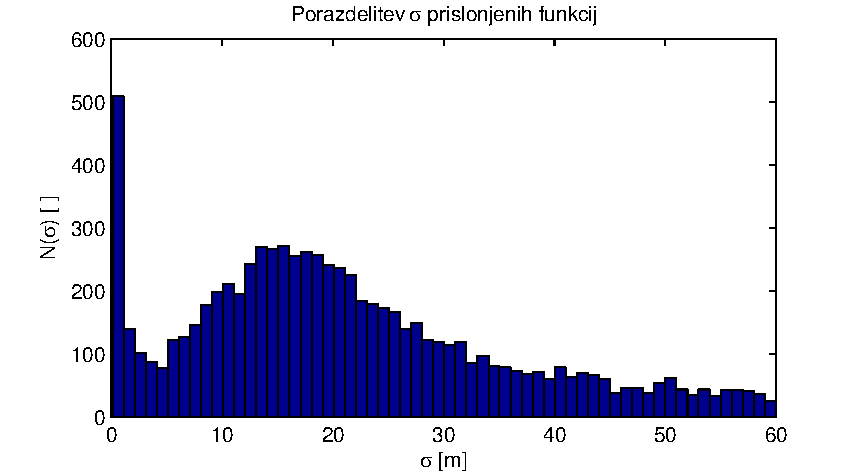
\includegraphics{slike/menisija-sigme-hist}
          \end{center}
          \caption{Porazdelitev uteži $\sigma$ za gaussovo funkcijo prilegano na vrtače v Menišiji}
          \label{fig:menisija-sigme-hist}
        \end{figure}

        Če na dobljene profile nalegamo eksponentno krivuljo (\ref{fit-profila}) in izrišemo odvisnost $\sigma_x (r_{eff})$, vidimo (Slika \ref{fig:menisija-sigma}).

        \begin{equation}
          f(r) = A \cdot e^{-\frac{(r-r_0)^2}{\sigma^2}} + C  
          \label{fit-profila}
        \end{equation}

        Odvisnost $\sigma_x(r_{eff})$ je iz naših podatkov težko določiti, zaenkrat poskusimo z linearno funkcijo (\ref{sigma-od-reff})

        \begin{equation}
          \sigma (r_{eff}) = k \cdot r_{eff} + C
          \label{sigma-od-reff}
        \end{equation}

        \begin{figure}[H]
          \centering
          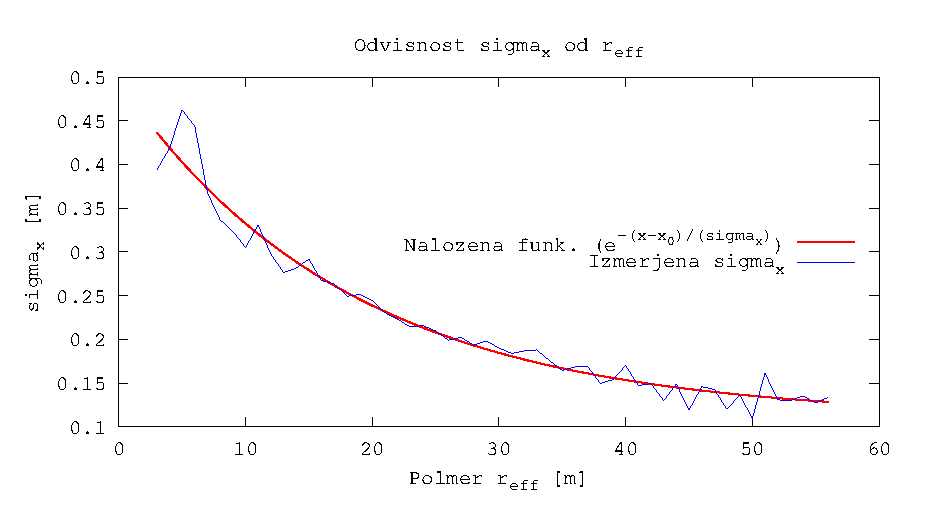
\includegraphics{slike/menisija-sigme}
          \caption{$\sigma$ s polmerom narašča}
          \label{fig:menisija-sigma}
        \end{figure}

        Na podlagi teh podatkov bi težko sklenili, da (\ref{fit-profila}) opiše profil idealne vrtače, a ujemanje je dobro in ga bomo uporabili za analitično modeliranje. 


        \chapter{Analitično modeliranje vrtač}
        \label{analiticno-modeliranje}

        \begin{comment}
        \section{Difuzijski model}

        Dinamiko vrtače poskusimo opisati z nelinearnimi difuzijsko enačbo (\ref{nelinearna-difuzijska-enacba}). V prejšnjem poglavju smo našli nastavek za stacionano stanje (\ref{ravnovesni-nastavek-vrtace}), ki ga dopolnimo še s časovnim delom (\ref{dinamicni-nastavek-vrtace}), ter predpostavimo difuzijsko konstanto (\ref{difuzijska-konstanta-1}). Privzamemo radialno simetričnost in računamo v cilindričnih koordinatah.

        \begin{equation}
          \frac{\partial z}{\partial t} = \nabla (K(z) \nabla z)
          \label{nelinearna-difuzijska-enacba}
        \end{equation}

        \begin{equation}
          z_0(r) = z(r,\infty) = Ae^{-\left(\frac{r}{\sigma }\right)^2}
          \label{ravnovesni-nastavek-vrtace}
        \end{equation}

        \begin{equation}
          z(r,t) = A e^{-\left(\frac{r}{\sigma }\right)^2} \left(1- e^{-\frac{t}{\tau }}\right)
          \label{dinamicni-nastavek-vrtace}
        \end{equation}

        \begin{equation}
          K(z) = -\frac{\sigma ^4}{4 r^2 \tau } \left(1-\frac{A}{z_0(r)}\right) \left(1-\frac{z_0(r)}{z(r,t)}\right)
          \label{difuzijska-konstanta-1}
        \end{equation}

        Vidimo, da je tok $\mathbf{j}$:
        \begin{equation}
          \mathbf{j} = -\frac{A \sigma^2}{2 r \tau } \left( 1-e^{-(\frac{r^2}{\sigma ^2})} \right) e^{-\frac{t}{\tau }}
          \label{tok}
        \end{equation}

        Ali zapisano z $z_0(r)$ in $z(r,t)$:
        \begin{equation}
          \mathbf{j} = - K(z) \nabla z(r,t) = \frac{\sigma^2}{2 r \tau} \left(1- \frac{A}{z_0(r)}\right) (z_0(r)-z(r,t))
        \end{equation}


        Izrišemo časovno dinamiko profila vrtače (\ref{dinamicni-nastavek-vrtace}) in toka (\ref{tok}) - (Slika \ref{fig:vrtaca-dinamicno} in \ref{fig:tok-dinamicno}) (vzamemo $A=-6,\sigma=5,\tau = 1$).


        Sedaj se postavimo daleč stran od centra vrtače, kjer po dolgem času velja:

        \begin{equation}
          \frac{\partial z}{\partial t} = -\frac{A e^{-\frac{(r \rightarrow \infty)^2}{\sigma ^2}-\frac{t \rightarrow \infty}{\tau }}}{\tau } = -\frac{A}{\tau} = v_{denudacije}
          \label{hitrost-denudacije}
        \end{equation}

        Ocenimo $\tau$ vrtač.

        \begin{equation}
          \tau = \frac{-A}{v_{denudacije}}=\frac{-5m}{-50\cdot 10^{-6} m/leto} = 10^5 leto
          \label{tau-vrtace}
        \end{equation}

        \begin{table}[H]
          \centering
          \begin{tabular}{| l | c | l | l |} \hline
            $\rho_r$ & $2700$ $kg/m^3$ & Gostota apnenca                                            \\ \hline
            $\rho_s$ & $1000$ $kg/m^3$ & Gostota delno preperele kamnine                            \\ \hline
            $C$      & $50 \cdot 10^{-6} m/leto$  & Hitrost preperevanja apnenca na ravnini         \\ \hline
            $K$      & $1 \cdot 10^{-4} m^2/leto$ & Difuzijska konstanta za delno preperelo kamnino \\ \hline
            $\sigma$ & $4.5m$ & $\sigma$ vrtače po nastavku (\ref{fit-profila})                     \\ \hline
            $A$      & $6m$ & Globina vrtače $A$ po nastavku (\ref{fit-profila})                    \\ \hline
          \end{tabular}
          \caption{Vrednosti iz literature \cite{Gams1967} \cite{ford2007karst} \cite{fleurant2008modelling} in \ref{realne-vrtace}. poglavja}
          \label{tab:tabela-konstant}
        \end{table}
        \end{comment}

        \begin{comment}
        \section{Dvofazni difuzijski model}

        Za izhodišče privzamemo difuzijski model, kot ga predlaga Heimsath \cite{Heimsath2001}.

        \begin{figure}[H]
          \centering
          \begin{tikzpicture}[
    scale=1.8,
    arrow/.style={thick,->,shorten <=-2pt, shorten >=-2pt},
    media/.style={font={\footnotesize\sffamily}}
]

    \fill[color=black!5] (0,4) coordinate (a_1) -- (6,2.5) coordinate (a_2) -- (6,0.5) coordinate (b_2) -- (0,2) coordinate (b_1)-- cycle;
    \fill[color=black!10] (b_1) -- (b_2) -- (6,0.2) coordinate (c_2) -- (0,1.7) coordinate (c_1) -- cycle;
    \fill[color=black!25] (c_1) -- (c_2) -- (6,0) -- (0,0) -- cycle;

    \path[media] (1,2.8) node [rotate=-13.5] {Delno preperela}
                            (1,2.5) node [rotate=-13.5] {kamnina, $\rho_s$}
                            (2,0.6) node [rotate=-13.5] {Nepreperela kamnina, $\rho_r$}
                            (1.3,1.5) node [rotate=-13.5] {Preperevanje};

    % Draw surface, solid rock boundary and dz_b
    \draw [thick]               (a_1) -- (a_2) node [above, xshift=-5pt] {$z$};
    \draw [thick]               (b_1) -- (b_2) node [above, xshift=-5pt] {$z_b$};
    \draw [dashed,thick] (c_1) -- (c_2);

    % Draw dr volume
    \draw (2,1.5) -- (2,3.5);
    \draw (4,1) -- (4,3);

    %Draw currents
    \draw [arrow] (1.75,2.4375) -- (2.25,2.3125) node [above=1pt] {$q_s(r)$};
    \draw [arrow] (3.75,1.9375) -- (4.25,1.8125) node [above left =9pt] {$q_s(r+dr)$};
    \draw [arrow] (2.5,1.25) -- (2.5,1.55) node [above] {$\rho_r \frac{\partial z_b}{\partial t}$};
    \draw [arrow] (3.5,1.3) -- (3.5,0.6) node [above=36] {$Q_s$};
    \draw [arrow] (3,3.1) -- (3,3.45) node [below=18pt] {$\rho_s \frac{\partial h}{\partial t}$};

    % Draw h and dz_b
    \draw [<->] (5,0.75) -- (5,2.75) node [midway, right] {$h$};
    \draw [<->] (5,0.45) -- (5,0.75) node [midway, right, yshift=-0pt,rotate=-13.5] {$dz_b$};

    % Draw axes
    \draw [<->,thick] (0,4.3) node (yaxis) [above] {$z$}
        |- (6.3,0) node (xaxis) [right] {$r$};

\end{tikzpicture}
          \caption{Skica difuzijskega modela nastajanja vrtače}
          \label{fig:difuzijski-model}
        \end{figure}

        \begin{equation}
          \rho_s \frac{\partial h}{\partial t} = -\rho_r \frac{\partial z_b}{\partial t} - \nabla q_s
          \label{kontinuitetna-enacba-original}
        \end{equation}

        Kjer je $h$ višina stolpca sedimenta, $z_b$ višina skalne podlage, $z$ višina površja, $\rho_r$ in $\rho_s$ gostoti skalne podlage in sedimenta, $q_s$ pa gostota toka sedimenta. Za gostoto toka sedimenta vzamemo, da je sorazmeren z naklonom površja:
        \begin{equation}
          q_s = - \rho_s K \nabla z
          \label{difuzijski-tok}
        \end{equation}

        Kjer je $K$ analogna konstanta difuzijski.
        Model dopolnimo z raztapljanjem in izpiranjem delno raztopljene kamnine v podzemlje - to pospravimo v člen $Q_s$ in vstavimo \ref{difuzijski-tok}.
        \begin{equation}
          \rho_s \frac{\partial h}{\partial t} = -\rho_r \frac{\partial z_b}{\partial t} + K \rho_s \Delta z - Q_s
          \label{kontinuitetna-enacba-1}
        \end{equation}

        Dobljen model skiciramo na (Slika \ref{fig:difuzijski-model}).

        V ravnovesnem stanju vrtače, ki smo ga domnevno našli v \ref{realne-vrtace}. poglavju (enačba \ref{fit-profila}) zahtevamo, da velja $\frac{\partial h}{\partial t} = 0$ in $\frac{\partial z_b}{\partial t} = C$, kjer $C<0$, saj se meja preperelosti znižuje. Dobimo:

        \begin{equation}
          Q_s = - \rho_r C + \rho_s K \Delta z
          \label{kontinuitetna-enacba-ravnovesje}
        \end{equation}

        Vstavimo ravnovesni profil vrtače (enačba \ref{fit-profila}) in vrednosti iz tabele (\ref{tab:tabela-konstant}), da dobimo profil $Q_s$ profil raztapljanja apnenca v na površju (Slika \ref{fig:profil-raztapljanja}).


        \begin{figure}[H]
          \begin{center}
            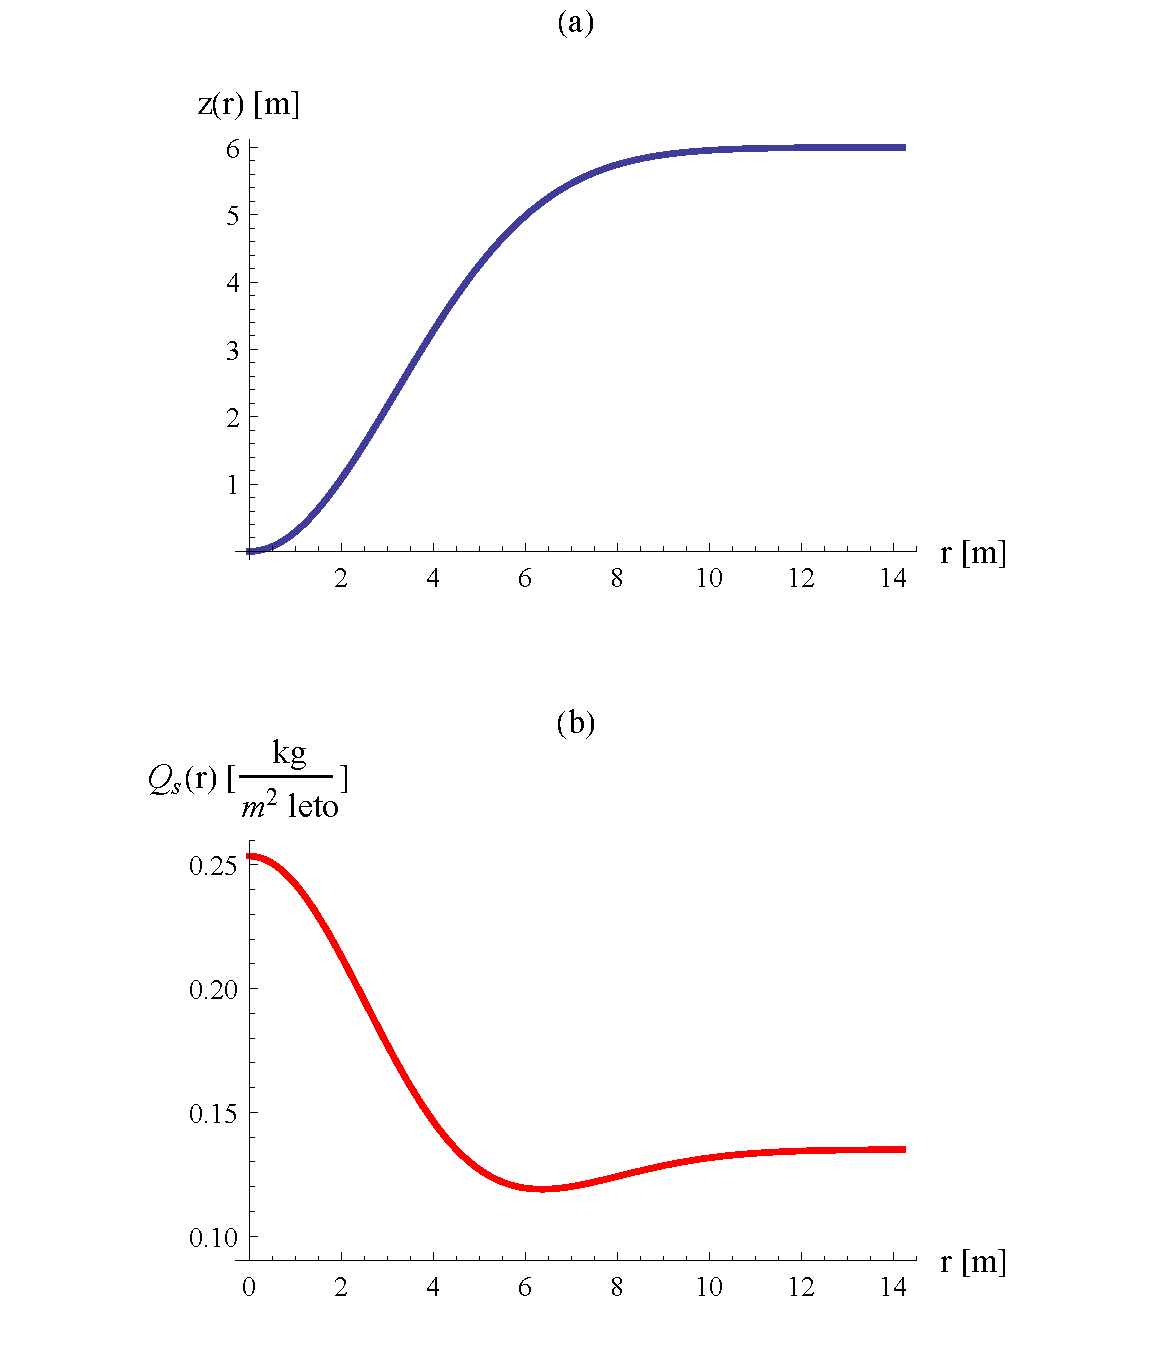
\includegraphics[width=10cm]{slike/profil-raztapljanja}
          \end{center}
          \caption{(a) Profil vrtače (b) modeliran profil raztapljanja delno preperele kamnine}
          \label{fig:profil-raztapljanja}
        \end{figure}

        Dobljeni profil raztapljanja nakazuje kvalitativno podobnost meritvam, ki jih je opravil Zambo (\cite{Zambo1997}) v osemdesetih (Slika \ref{fig:vrtaca-aggtelek}).

        \begin{figure}[H]
          \begin{center}
            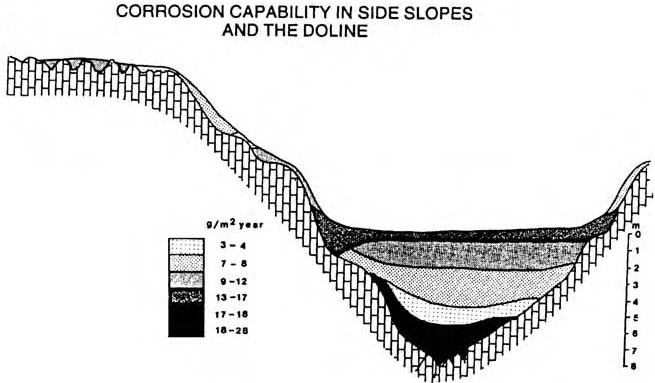
\includegraphics[width=10cm]{slike/vrtaca-aggtelek}
          \end{center}
          \caption{Meritve raztapljanja apnenca v realni vrtači - dolina Beke, nacionalni park Aggtelek na Madžarskem \cite{Zambo1997}}
          \label{fig:vrtaca-aggtelek}
        \end{figure}

        Profil vrtače blizu ravnovesja zmotimo s spremembo vrednosti oblike profila ($z(r)$), vstavimo nastavek za $\frac{\partial z_b}{\partial t}=\frac{1}{|h_0-h|}$ in \dots

        \end{comment}


        \section{Stohastična rast površin}
        \label{definicije}

        Za opis področja vrtač uporabimo analogijo z rastjo vmesnikov - npr. nabiranjem vodnega kamna - le da tu nebo raste v apnenčasto podlago.
        Po \cite{barabasi1995fractal} v poglavju (\ref{definicije}) povzamemo definicije potrebne za opis takega procesa.
        Povprečna višina površja je definirana kot \ref{povprecna-visina}, kjer je $h(i,t)$ višina stolpca $i$ ob času $t$.

        \begin{equation}
          \bar{h} = \frac{1}{L} \sum_{i=1}^L h(i,t)
          \label{povprecna-visina}
        \end{equation}

        Če je hitrost usedanja delcev konstantna, se povprečna višina povečuje linearno s časom $\bar{h}(t) \sim t$.

        Širino vmesnika, ki poda hrapavost vmesnika, definiramo s standardnim odklonom višine vmesnika od povprečne višine:

        \begin{equation}
          w(L,t) = \sqrt{\frac{1}{L} \sum_{i=1}^L (h(i,t)-\bar{h}(t))^2}
          \label{sirina-vmesnika}
        \end{equation}

        (\ref{sirina-vmesnika}) spremljamo v času, da lahko kvantitativno podamo hrapavost površine. Po definiciji začnemo z ravnim vmesnikom in širino 0. V začetku $(t \ll t_x)$ se nam širina povečuje eksponentno s časom:

        \begin{equation}
          w(L,t) \sim t^\beta
          \label{beta}
        \end{equation}

        kjer je $\beta$ exponent rasti, ki poda časovno dinamiko hrapavosti.
        Po dolgem času $(t \gg t_x)$ širina vmesnika preide v zasičeni režim, v katerem se eksponentna rast ustavi in doseže zasičeno vrednost $w_{sat}$, ki je odvisna od velikosti sistema $L$ takole:

        \begin{equation}
          w_{sat}(L) \sim L^\alpha
          \label{alfa}
        \end{equation}

        Eksponent $\alpha$ imenujemo eksponent hrapavosti, in nam poda hrapavost nasičenega vmesnika.

        Prehodni čas $t_x$, okoli katerega vmesnik preide iz nezasičenega v zasičen režim, je odvisen od velikosti sistema in je približno:

        \begin{equation}
          t_x \sim L^z
          \label{z}
        \end{equation}

        kjer je $z$ dinamični eksponent.
        Eksponenti $\alpha$, $\beta$ in $z$ med seboj niso neodvisni.
        Izkaže se, da z izrisom $w(L,t)/w_{sat}(L)$ kot funkcije časa, dobimo krivulje, ki se zasitijo ob istem času, ne glede na velikost sistema $L$.
        Če izrišemo širino vmesnika kot funkcijo $t/t_x$, se bodo vse krivulje zasitile v isti točki.
        Zato sklepamo, da je $w(L,t)/w_{sat}(L)$ funkcija $t/t_x$, torej:

        \begin{equation}
          \frac{w(L,t)}{w_{sat}(L)} \sim f(\frac{t}{t_x})
        \end{equation}

        kjer je $f(u)$ funkcija lestvičenja in če nadomestimo $w_{sat}$ in $t_x$, dobimo Family-Vicsek relacijo lestvičenja:

        \begin{equation}
          w(L,t) \sim L^\alpha f(\frac{t}{L^z})
          \label{family-vicsek}
        \end{equation}

        Za $f(u)$ velja:
        \begin{equation}
          f(u) \propto \left \{ \begin{array}{lr} u^{\beta} & \ u\ll 1 \\
            1 & \ u\gg1\end{array} \right. 
        \end{equation}

            Če sedaj izrišemo več različnih razvojev površja na en graf ((Slika \ref{fig:barabasi}) iz \cite{barabasi1995fractal}), dobimo jasnejšo predstavo o funkciji lestvičenja. Če se točki $(t_x,w(t_x))$ približamo z leve, vidimo, da po (\ref{beta}) velja $w(t_x) \sim t_x^\beta$. Hkrati pa, da če se isti točki približujemo z desne po (\ref{alfa}) velja $w(t_x) \sim L^\alpha$. Torej $t_x^\beta \sim L^\alpha$ in po (\ref{z}) sledi zakon o lestvičenju:

            \begin{equation}
              z = \frac{\alpha}{\beta}
            \end{equation}

            \begin{figure}[H]
              \begin{center}
                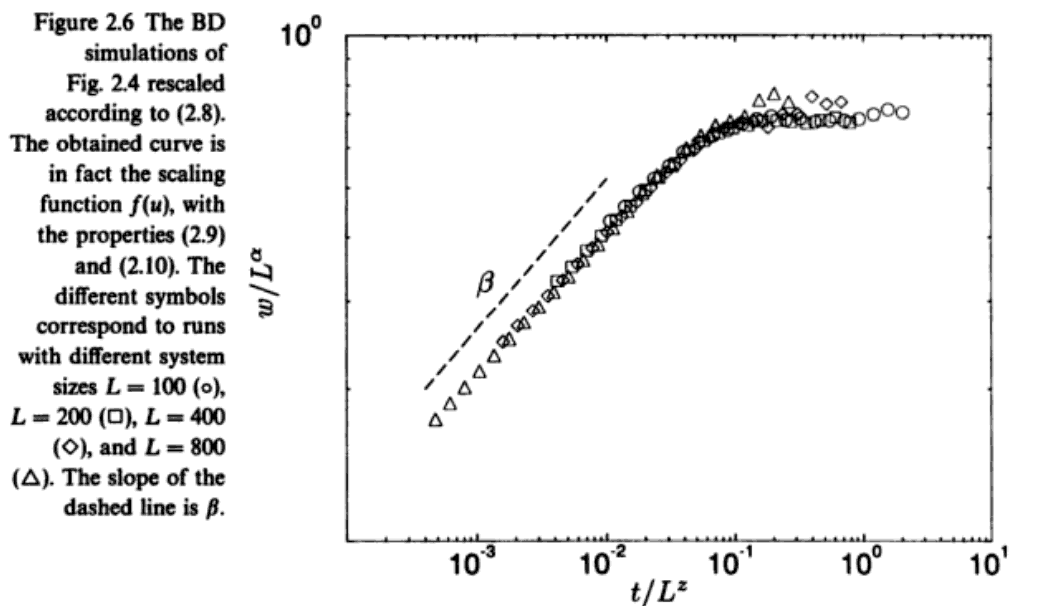
\includegraphics[width=13cm]{slike/barabasi}
              \end{center}
              \caption{Simulirane vrednosti širine vmesnika pri naključnem usedanju, za različne velikosti vmesnika \cite{barabasi1995fractal}}
              \label{fig:barabasi}
            \end{figure}



            \section{Merjenje eksponenta hrapavosti}
            \label{hrapavost}

            Zvezo (\ref{alfa}) predelamo  v $ w_{sat}=C \cdot L^\alpha $ in dobimo:

            \begin{equation}
              \alpha = \frac{\partial ( ln (w_{sat}) ) }{\partial ( ln L )}
              \label{alpha-numeric}
            \end{equation}

            Na Lidar modelu Menišije uporabljenem v (Poglavje \ref{realne-vrtace}) izračunamo $\bar{w}_{sat}$ za vmesnike, kjer je L med 5 in 10 km. Širine vmesnikov $w$ nato narišemo v odvisnosti od velikosti vmesnika L.

            Dobimo graf (Slika \ref{fig:menisija-alfa}) s katega odberemo, da je $\alpha =  0.4368 \pm 0.0005$.

            \begin{figure}[H]
              \begin{center}
                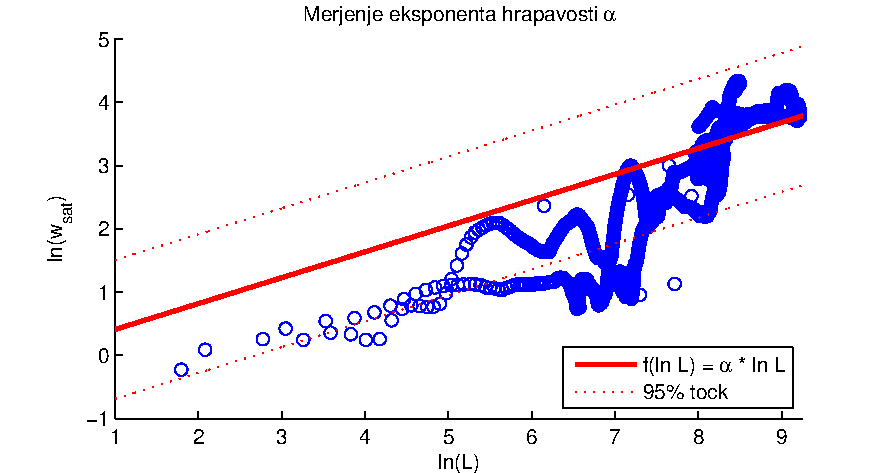
\includegraphics{slike/menisija-alfa.pdf}
              \end{center}
              \caption{Prileganje premice $f(ln(L)) = \alpha \cdot x$ h krivulji $ln(w_{sat}(ln(L)))$ nam poda eksponent hrapavosti}
              \label{fig:menisija-alfa}
            \end{figure}


            \section{Model Kardar-Parisi-Zhang}

            Za modeliranje procesa nastanka vrtač lahko vzamemo, da kamnina razpada stohastično kot $\eta(\mathbf{x},t)$, ki je bel Gaussov šum, za katerega velja: $ \langle \eta(\mathbf{x},t) \rangle=0 $ in
        \begin{equation}
            \langle \eta(\mathbf{x},t) \eta(\mathbf{x'},t')\rangle = 2 D \delta^d(\mathbf{x}-\mathbf{x'})(t-t')
        \end{equation}

            Ko se del kamnine raztopi, pomaknemo površino površja v smeri normale (Slika \ref{fig:kpz}), torej se površje v smeri osi h v času $\delta t$ pomakne za 
        \begin{equation}
          \delta h = \sqrt{ (v \delta t)^2 + (v \delta t \nabla h)^2}
        \end{equation}

        Če je $|\nabla h| \ll 1$, dobimo: 
        \begin{equation}
            \dot h = v \sqrt{1 + (\nabla h)^2} \simeq v + \frac{v}{2} (\nabla h)^2 + \ldots
        \end{equation}

            \begin{figure}[H]
              \begin{center}
                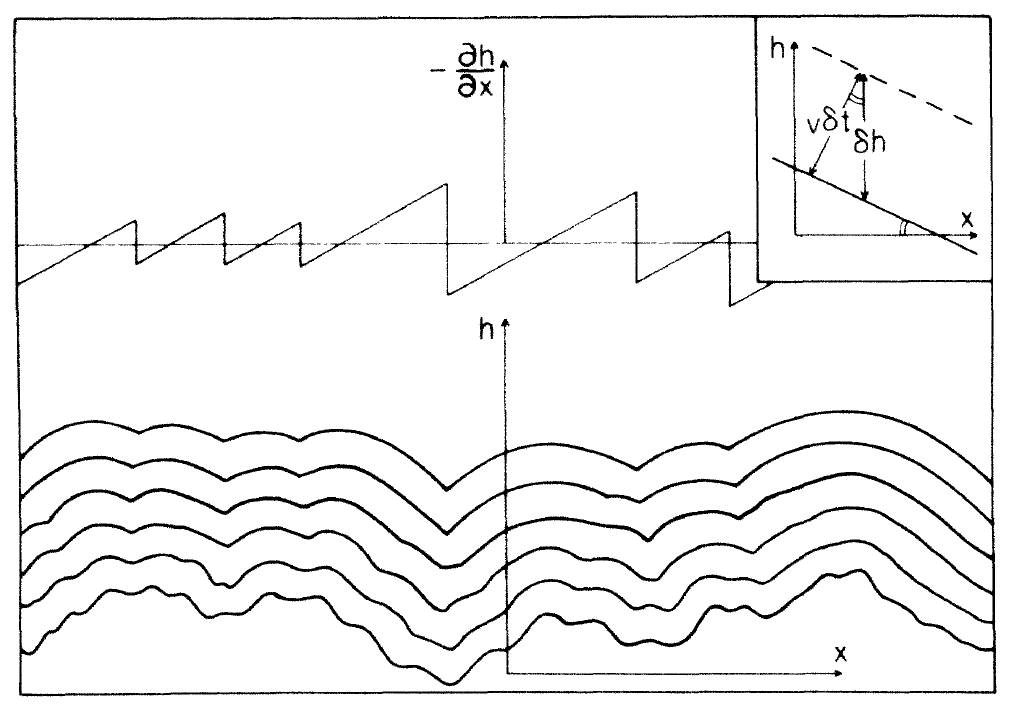
\includegraphics[width=10cm]{slike/kpz}
              \end{center}
              \caption{Zaporedni profili deterministične rasti, priraščanje v smeri normale površja je prikazano desno zgoraj}
              \label{fig:kpz}
            \end{figure}

            To nam da člen $\frac{\lambda}{2} (\nabla h)^2$.

            Vzamemo, da zaradi počasnosti procesa prihaja do difuzije površja in dodamo člen $\nu \nabla^2 h$.

            Sestavljeni nam ti členi dajo Kardar-Parisi-Zhang enačbo (\cite{kardar1986dynamic}):

            \begin{equation}
              \frac{\partial h}{\partial t} = \nu \nabla^2 h + \frac{\lambda}{2} (\nabla h)^2 + \eta (\mathbf{x},t)
              \label{KPZ}
            \end{equation}

            Vzamemo nastavek:
        \begin{equation}
            h(\mathbf{x},t) = \frac{2 \nu}{\lambda} log(Z(\mathbf{x},t))
        \end{equation}
            in dobimo stohastično difuzijsko enačbo:

        \begin{equation}
            \frac{\partial Z}{\partial t} = \nu \nabla^2 Z + \frac{\lambda}{2 \nu} \eta(\mathbf{x},t) Z
        \end{equation}

        katere rešitev je:
        \begin{equation}
            h(\mathbf{x},t) = \frac{2 \nu}{\lambda} ln \left( \int_{-\infty}^{\infty} \frac{d^d \xi}{(4 \pi \nu t)^{d/2}} \cdot exp \left[-\frac{(x-\xi)^2}{4 \nu t} + \frac{\lambda}{2 \nu}h(\xi,0) \right] \right)
        \end{equation}

            \cite{kardar1986dynamic} nato v fourierovem prostoru s prostim propagatorjem in pogojem za beli šum perturbativno rešijo (\ref{KPZ}). Končno pokažejo, da za stohastično priraščanje površja velja: $z = \frac{3}{2}$ in $\alpha=\frac{1}{2}$. To se relativno dobro ujema z $\alpha=0.4368 \pm 0.0005$ namerjenim v (Poglavje \ref{hrapavost}).


            Če simuliramo stohastično rast površja, opazimo, da je končno stanje površja modela precej stabilno, a ne ravnovesno in precej odvisno od začetnih pogojev. Oblike, ki na površju nastanejo, so si med seboj podobne po obliki in velikosti. (Slika \ref{fig:KPZ-numericno}) je primer tako simuliranega površja.

            \begin{figure}[H]
              \begin{center}
                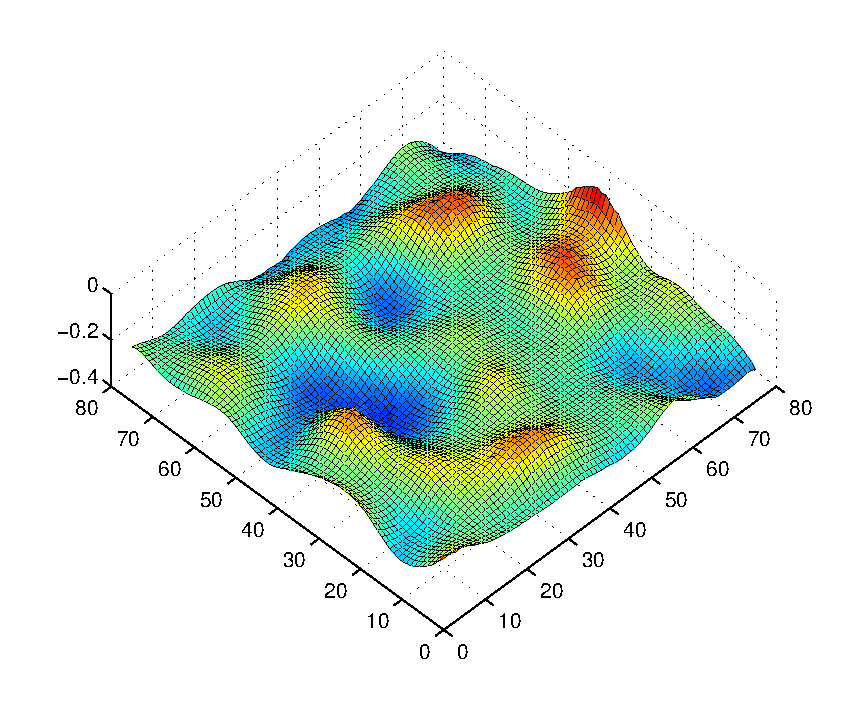
\includegraphics[width=13cm]{slike/KPZ-numericno}
              \end{center}
              \caption{Numerična simulacija po Kardar-Parisi-Zhang enačbi razvijajočega se površja po $10^5$ korakih}
              \label{fig:KPZ-numericno}
            \end{figure}


            \section{Modeliranje dinamike vrtač}

            Za modeliranje dinamike posamezne vrtače stohastični procesi niso primerni, zato si za opis pogledamo dinamično enačbo (\ref{dinamicna-splosna}) z različnimi variacijami člena rasti $F(h)$ (\ref{dinamicna-variacije}). Izbor enačb je povzet po \cite{kandler2010population}.

            \begin{equation}
              \frac{ \partial h(t,x) }{ \partial t} = F(h)
              \label{dinamicna-splosna}
            \end{equation}

          \begin{equation}
            F(h) = \left \{ \begin{array}{lr} 
            a \cdot h \\
            a \cdot h \cdot (1 - \frac{h}{K}) \\
            a \cdot (K - h) \\
            - h \cdot e^{-a t}
            \end{array} \right. 
            \label{dinamicna-variacije}
          \end{equation}

          \subsection{Eksponentna rast}

          V modelu eksponentne rasti predpostavimo, da je rast sorazmerna z vrdnosjo ($h(t)$) v izbrani točki. Dobimo enačbo (\ref{dinamicna-eksponentna}), ki jo reši funkcija (\ref{dinamicna-eksponentna-resitev}), in jo pri variaciji parametra $a$ narišemo (Slika \ref{fig:eksponentna-rast}).

          \begin{equation}
            \frac{\partial h(t)}{\partial t} = a \cdot h(t)
            \label{dinamicna-eksponentna}
          \end{equation}

          \begin{equation}
            h(t) = h_0 e^{a t}
            \label{dinamicna-eksponentna-resitev}
          \end{equation}

          \begin{figure}[h]
            \begin{center}
              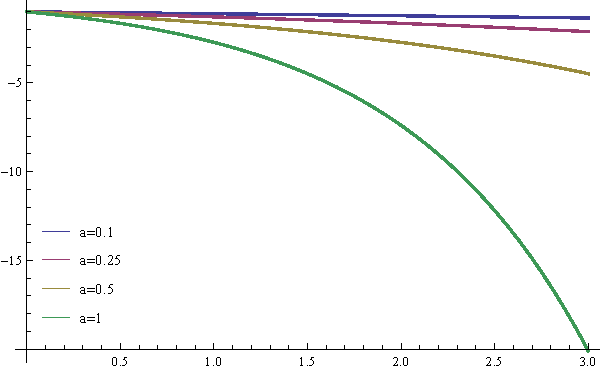
\includegraphics[width=9cm]{slike/eksponentna-rast}
            \end{center}
            \caption{Vzeli smo začetno vrednost $h_0 = -1$ in variirali vrednost $a$. \newline $a=0,1;0,25;0,5;1$}
            \label{fig:eksponentna-rast}
          \end{figure}

          Če je parameter $a > 0$, bomo vedno dobili neomejeno rast, kar zmanjšuje splošnost tega modela. Vseeno pa je v omejenih intervalih uporaben za npr. opis rasti populacij držav, širjenje virusov, jedrskih verižnih reakcij, itn. Uporabnost modela se konča, ko se sistem zasiti - to je, ko zmanjka virov, ki rast poganjajo (če gledamo dane primere - ko zmanjka hrane, celic, jeder).
          Pri vrtačah je možno, da imamo eksponento rast v začetku, a tega ne moremo ne dokazati ne ovreči. Vsekakor pa je ni v ravnovesni fazi, saj zelo globokih vrtač ne opazimo.


          \subsection{Logistična rast}

          V model logistične rasti predpostavimo, da je rast sorazmerna z višino v izbrani točki, ter da se zmanjšuje, ko se približujemo fizikalnim omejitvam sistema (npr. pomanjkanju hrane, življenskega prostora, itn). To zapšemo v enačbo (\ref{dinamicna-logisticna}), ki jo reši funkcija (\ref{dinamicna-logisticna-resitev}).

          \begin{equation}
            \frac{\partial h(t)}{\partial t} = a \cdot \left( 1 - \frac{h(t)}{K} \right) h(t)
            \label{dinamicna-logisticna}
          \end{equation}

            \begin{equation}
            h(t) = \frac{h_0 K e^{a t}}{K + h_0 (e^{a t}-1)}
            \label{dinamicna-logisticna-resitev}
          \end{equation}

            \begin{figure}[h]
              \begin{center}
                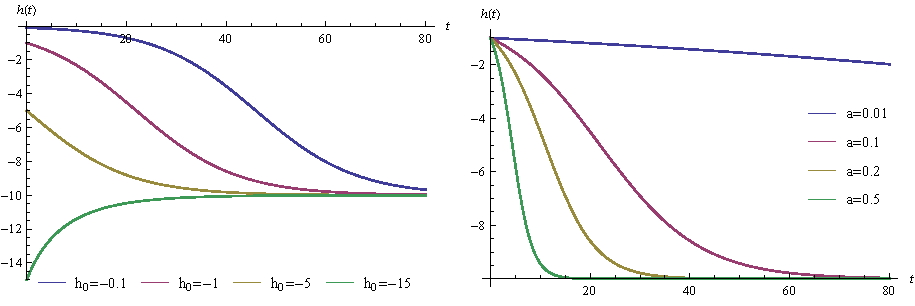
\includegraphics[width=14cm]{slike/logisticna-rast}
              \end{center}
              \caption{Logistična rast po (\ref{dinamicna-logisticna-resitev}). Vzeli smo $K=-10$ in variirali ostale parametre. V prvem primeru smo pri $a=0,1$ vzeli $h_0=-0,1;-1;-5;-15$. V drugem pa pri $h_0=-1$, $a=0.01;0.1;0.2;0,5$}
              \label{fig:logisticna-rast}
            \end{figure}

          Vidimo, da neglede na izbiro začetne točke $h_0$, vrednost h(t) konvergira proti vrednosti $K$. Torej je rast omejena s kapaciteto sistema K.
          Če funkcijo (\ref{dinamicna-logisticna-resitev}) Taylorjevo razvijemo, vidimo, da je rast, kjer $h(t) \ll K$, približno $a h(t)$. V območju, kjer je $h(t)$ bližji $K$, pa postane drugi člen v razvoju $-a h(t)^2 / K$ pomembnejši in rast se po dolgem času ustavi.
          Model logistične rasti se uporablja za modeliranje človeških in živalskih populacij, rasti tumorjev, širjenje inovacij v družbi in sprememb v jeziku. Zaradi omejene rasti pa se zdi tudi zanimiv kandidat za modeliranje dinamike vrtač.


          \subsection{Omejena eksponentna rast}

          Model omejene eksponentne rasti pravi, da je rast tem večja, čim dlje smo od omejitve sistema $K$ in vedno v smeri proti vrednosti $K$. To zapišemo v enačbo (\ref{dinamicna-omejena-eksponentna}) in rešimo z (\ref{dinamicna-omejena-eksponentna-resitev}).

          \begin{equation}
            \frac{\partial h(t)}{\partial t} = a \cdot ( K - h(t) ) = a K - a h(t)
            \label{dinamicna-omejena-eksponentna}
          \end{equation}

          Rešitev pa je
          \begin{equation}
            h(t) = K - (K - h_0) e^{-a t}
            \label{dinamicna-omejena-eksponentna-resitev}
          \end{equation}

            Medtem ko je omejena eksponentna rast podobna logistični, pa ima logistična v začetku položnejšo rast. Omejena eksponentna rast se uporablja za modeliranje sistemov, v katerih dinamiko poganjajo zunanji dejavniki in znotraj katerih ni interakcij. Naprimer pri širjenju inovacij v družbi.

            \begin{figure}[H]
              \begin{center}
                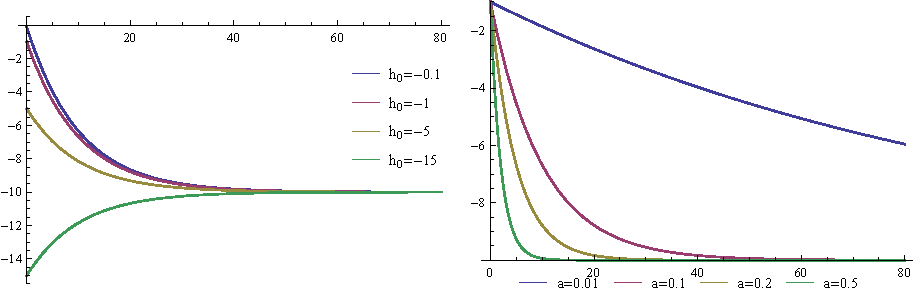
\includegraphics[width=14cm]{slike/omejena-eksponentna-rast}
              \end{center}
              \caption{Omejena eksponentna rast po (\ref{dinamicna-omejena-eksponentna-resitev}). Vzeli smo $K=-10$ in variirali ostale parametre. V prvem primeru smo pri $a=0,1$ vzeli $h_0=-0,1;-1;-5;-15$. V drugem pa pri $h_0=-1$, $a=0.01;0.1;0.2;0,5$}
              \label{fig:omejena-eksponentna-rast}
            \end{figure}



          \subsection{Gompertzova rast}

          Pri modelu Gompertzove rasti vzamemo, da se faktor rasti s časom spreminja po enačbi (\ref{dinamicna-gompertzova-faktor}), kar nam da enačbo (\ref{dinamicna-gompertzova}) in rešitev (\ref{dinamicna-gompertzova-resitev}), iz katere lahko dobimo še asimptotsko rešitev (\ref{dinamicna-gompertzova-faktor}), ki je podobna zasičenosti modela pri prejšnih dveh primerih, a nastopi zaradi postopnega prenehanja rasti, in ne zaradi povratne zanke (kot v primeru logistične in omejene eksponentne rasti).

          \begin{equation}
            a(t) = a_0 \cdot e^{- k t}
            \label{dinamicna-gompertzova-faktor}
          \end{equation}

          \begin{equation}
            \frac{\partial h(t)}{\partial t} = a(t) \cdot h(t) = a_0 e^{ -k t} h(t)
            \label{dinamicna-gompertzova}
          \end{equation}

          \begin{equation}
            h(t) = h_0 \cdot e^{\frac{a_0}{k}(1-e^{-kt})}
           \label{dinamicna-gompertzova-resitev}
          \end{equation}

          \begin{equation}
            h(t) = h_0 \cdot e^{\frac{a_0}{k}} \quad \text{pri} \quad t \rightarrow \infty
            \label{dinamicna-gompertzova-limita}
          \end{equation}

            \begin{figure}[H]
              \begin{center}
                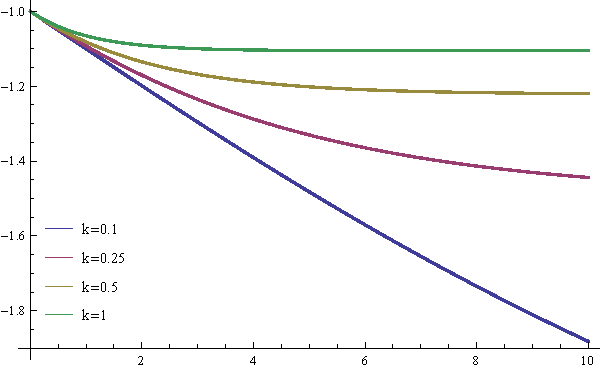
\includegraphics[width=9cm]{slike/gompertzova-rast}
              \end{center}
              \caption{Vzeli smo $h_0=-1$ in $a_0=0,1$ in variirali $k=0,1;0,25;0,5;1$}
              \label{fig:gompertzova-rast}
            \end{figure}

            \section{Difuzijsko modeliranje dinamike vrtač}

            Zaradi počasnosti procesa, ki oblikuje vrtače, domnevamo, da difuzija ni nepomembna, in dodamo dinamičnim modelom iz prejšnega podpoglavja  (\ref{difuzijska-variacije}) še difuzijski člen (\ref{difuzija-splosna}).

            \begin{equation}
              \frac{ \partial h(t,x) }{ \partial t} = D \Delta h(t.x) + F(h)
              \label{difuzija-splosna}
            \end{equation}

          \begin{equation}
            F(h) = \left \{ \begin{array}{lr} 
            a \cdot h \\
            a \cdot h \cdot (1 - \frac{h}{K}) \\
            a \cdot (K - h) \\
            - h \cdot e^{-a t}
            \end{array} \right. 
            \label{difuzijska-variacije}
          \end{equation}

          Rešitve teh enačb bomo iskali numerično in komentirali njihovo časovno dinamiko. Vzeli bomo sledeče robne pogoje:

        \begin{equation}
          \begin{aligned}
            h(0,x) =  - e^{-x^2}, x \in D \\
            h(t,x) = 0, x \in \partial D \\
            \frac{\partial h(t,x)}{\partial n} = 0, x \in \partial D \\
          \end{aligned}
        \end{equation}


          \subsection{Eksponentna rast}

            \begin{equation}
              \frac{ \partial h(t,x) }{ \partial t} = D \Delta h(t.x) + a \cdot h(t,x)
              \label{difuzija-eksponentna-rast}
            \end{equation}

            Sistem nam da eksponentno rast, kot je prikazano na (Slika \ref{fig:difuzija-eksponentna-rast}).

            \begin{figure}[H]
              \begin{center}
                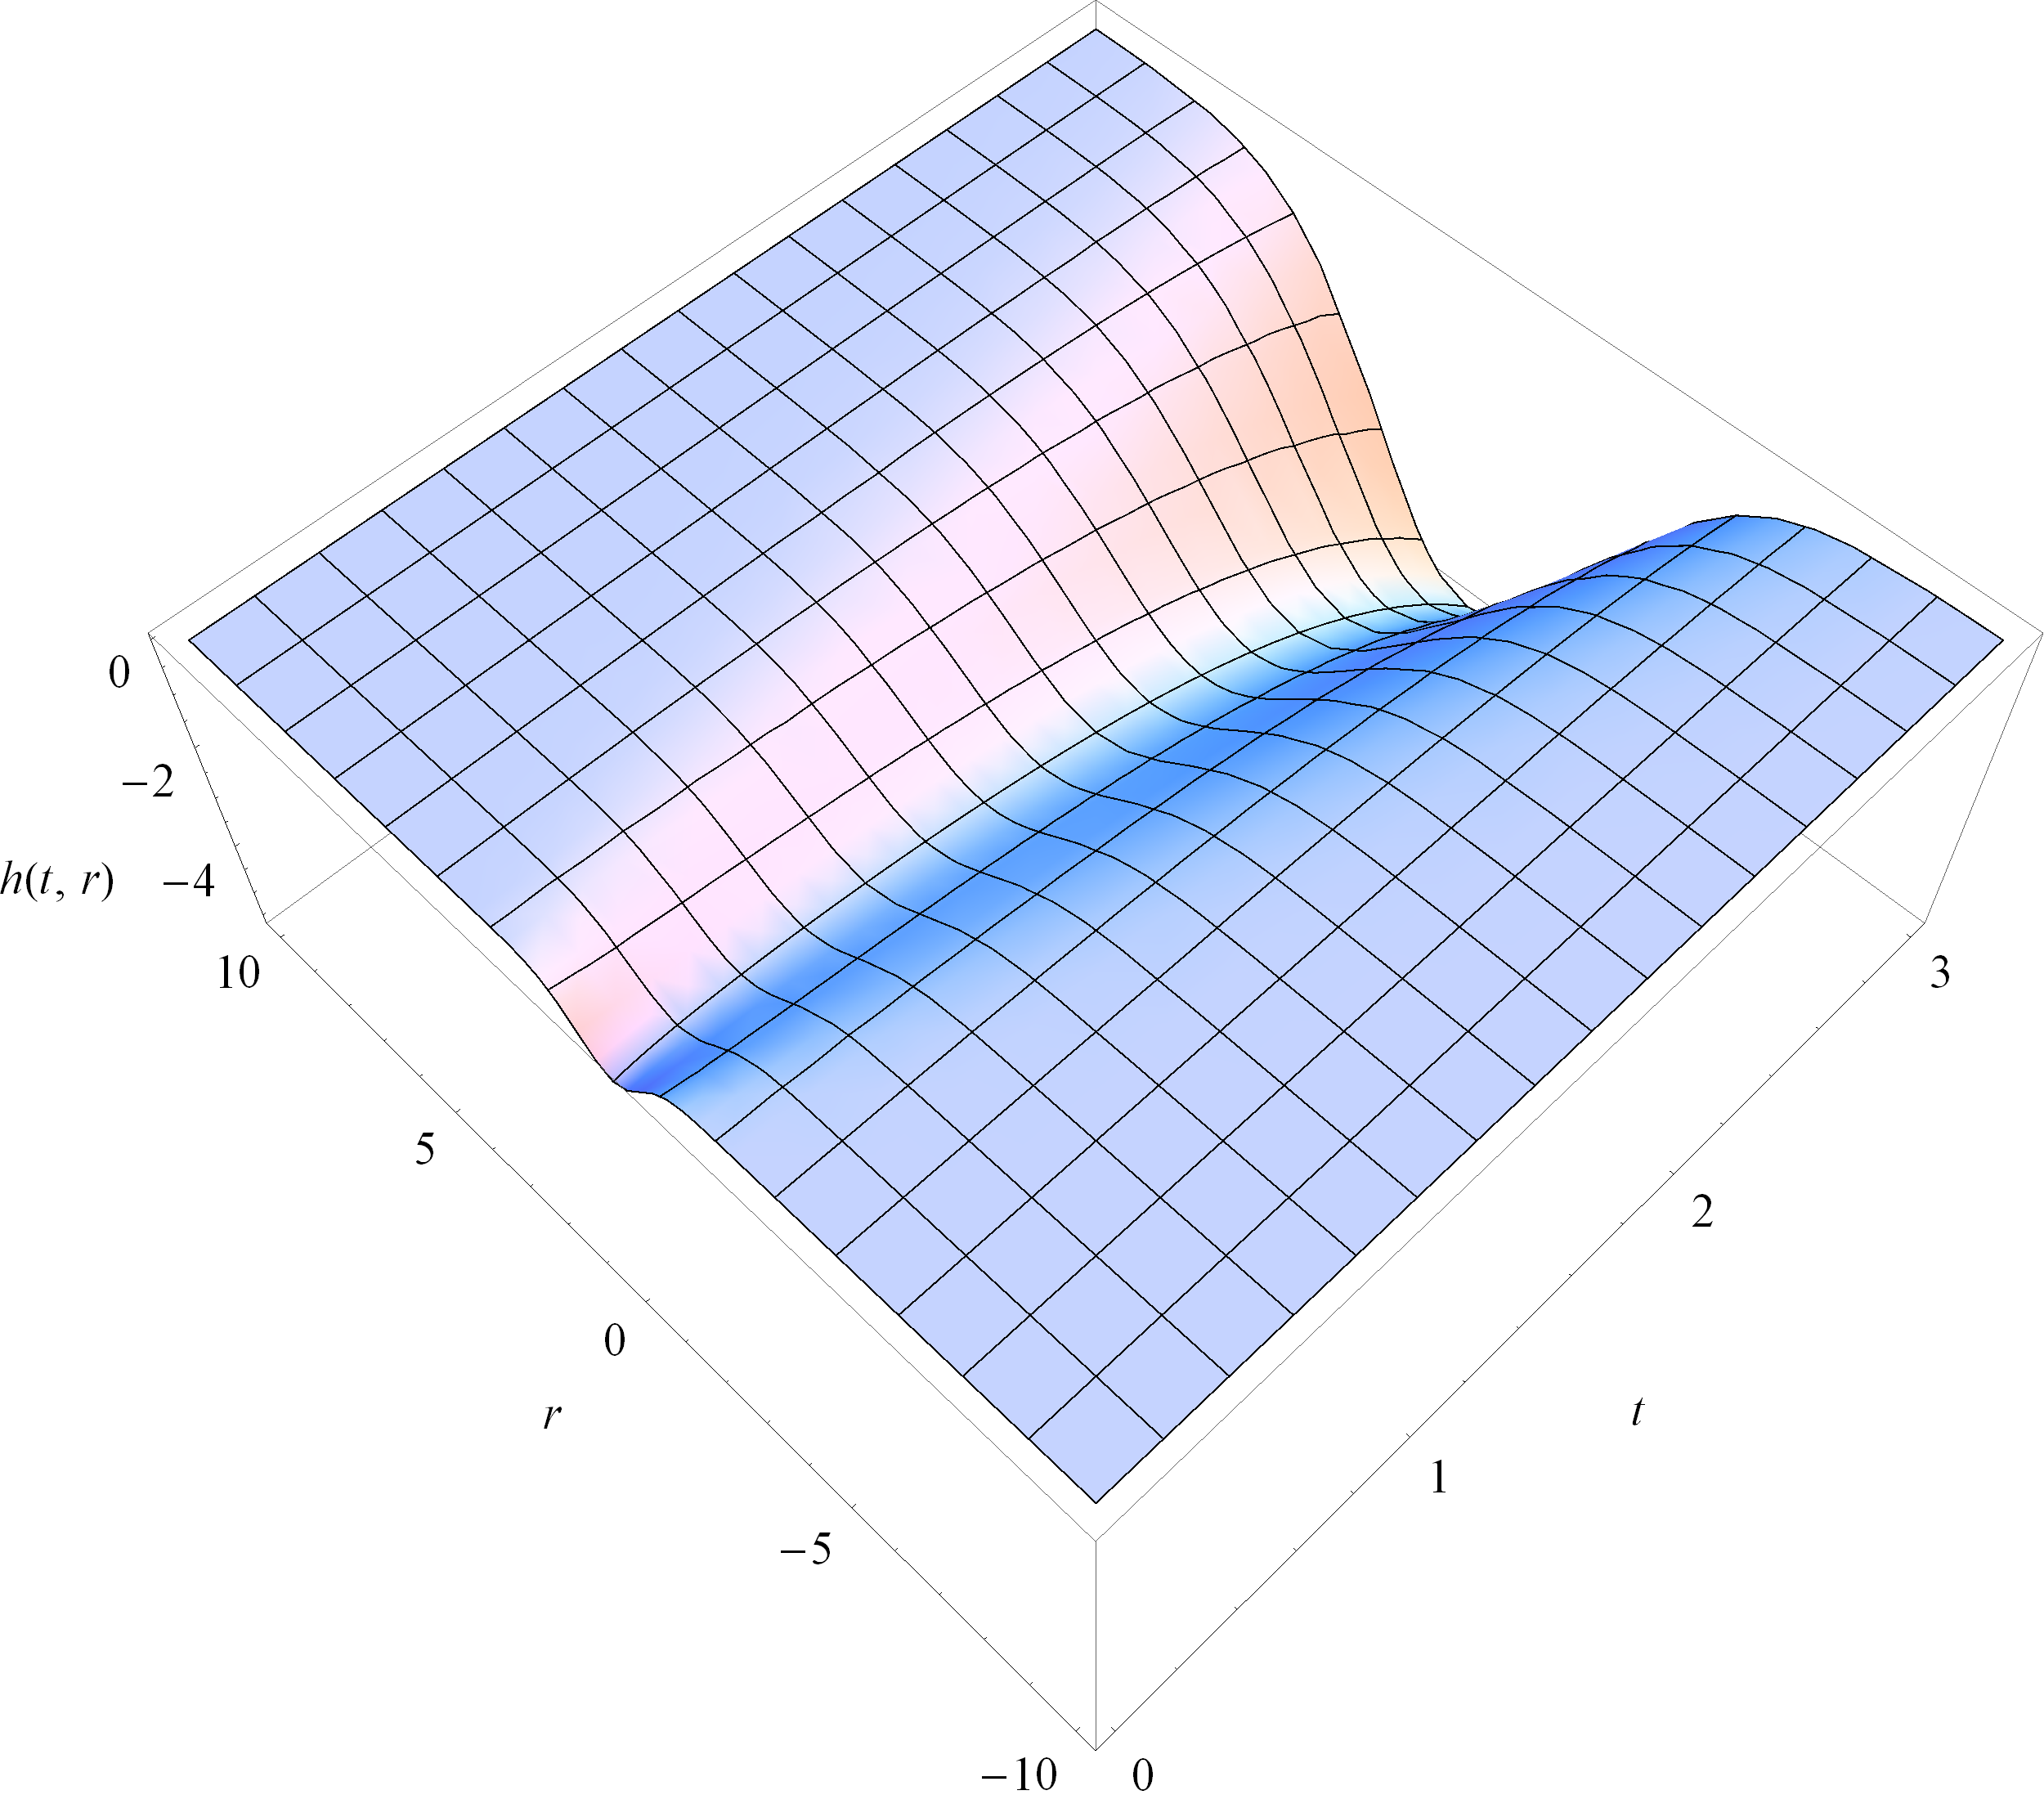
\includegraphics[width=10cm]{slike/difuzija-eksponentna-rast2}
              \end{center}
              \caption{Vzeli smo $D=1$, $a=1$}
              \label{fig:difuzija-eksponentna-rast}
            \end{figure}

            Eksponentna rast za vrtače ni primeren model, saj zelo velikih vrtač v naravi ne opazimo.


          \subsection{Logistična rast}

            Dobimo t.i. Fisher-Kolmogorovo enačbo:

            \begin{equation}
              \frac{ \partial h(t,x) }{ \partial t} = D \Delta h(t.x) + a \cdot h(t.x) \cdot (1 - \frac{h(t.x)}{K})
              \label{difuzija-logisticna-rast}
            \end{equation}

            \begin{figure}[H]
              \begin{center}
                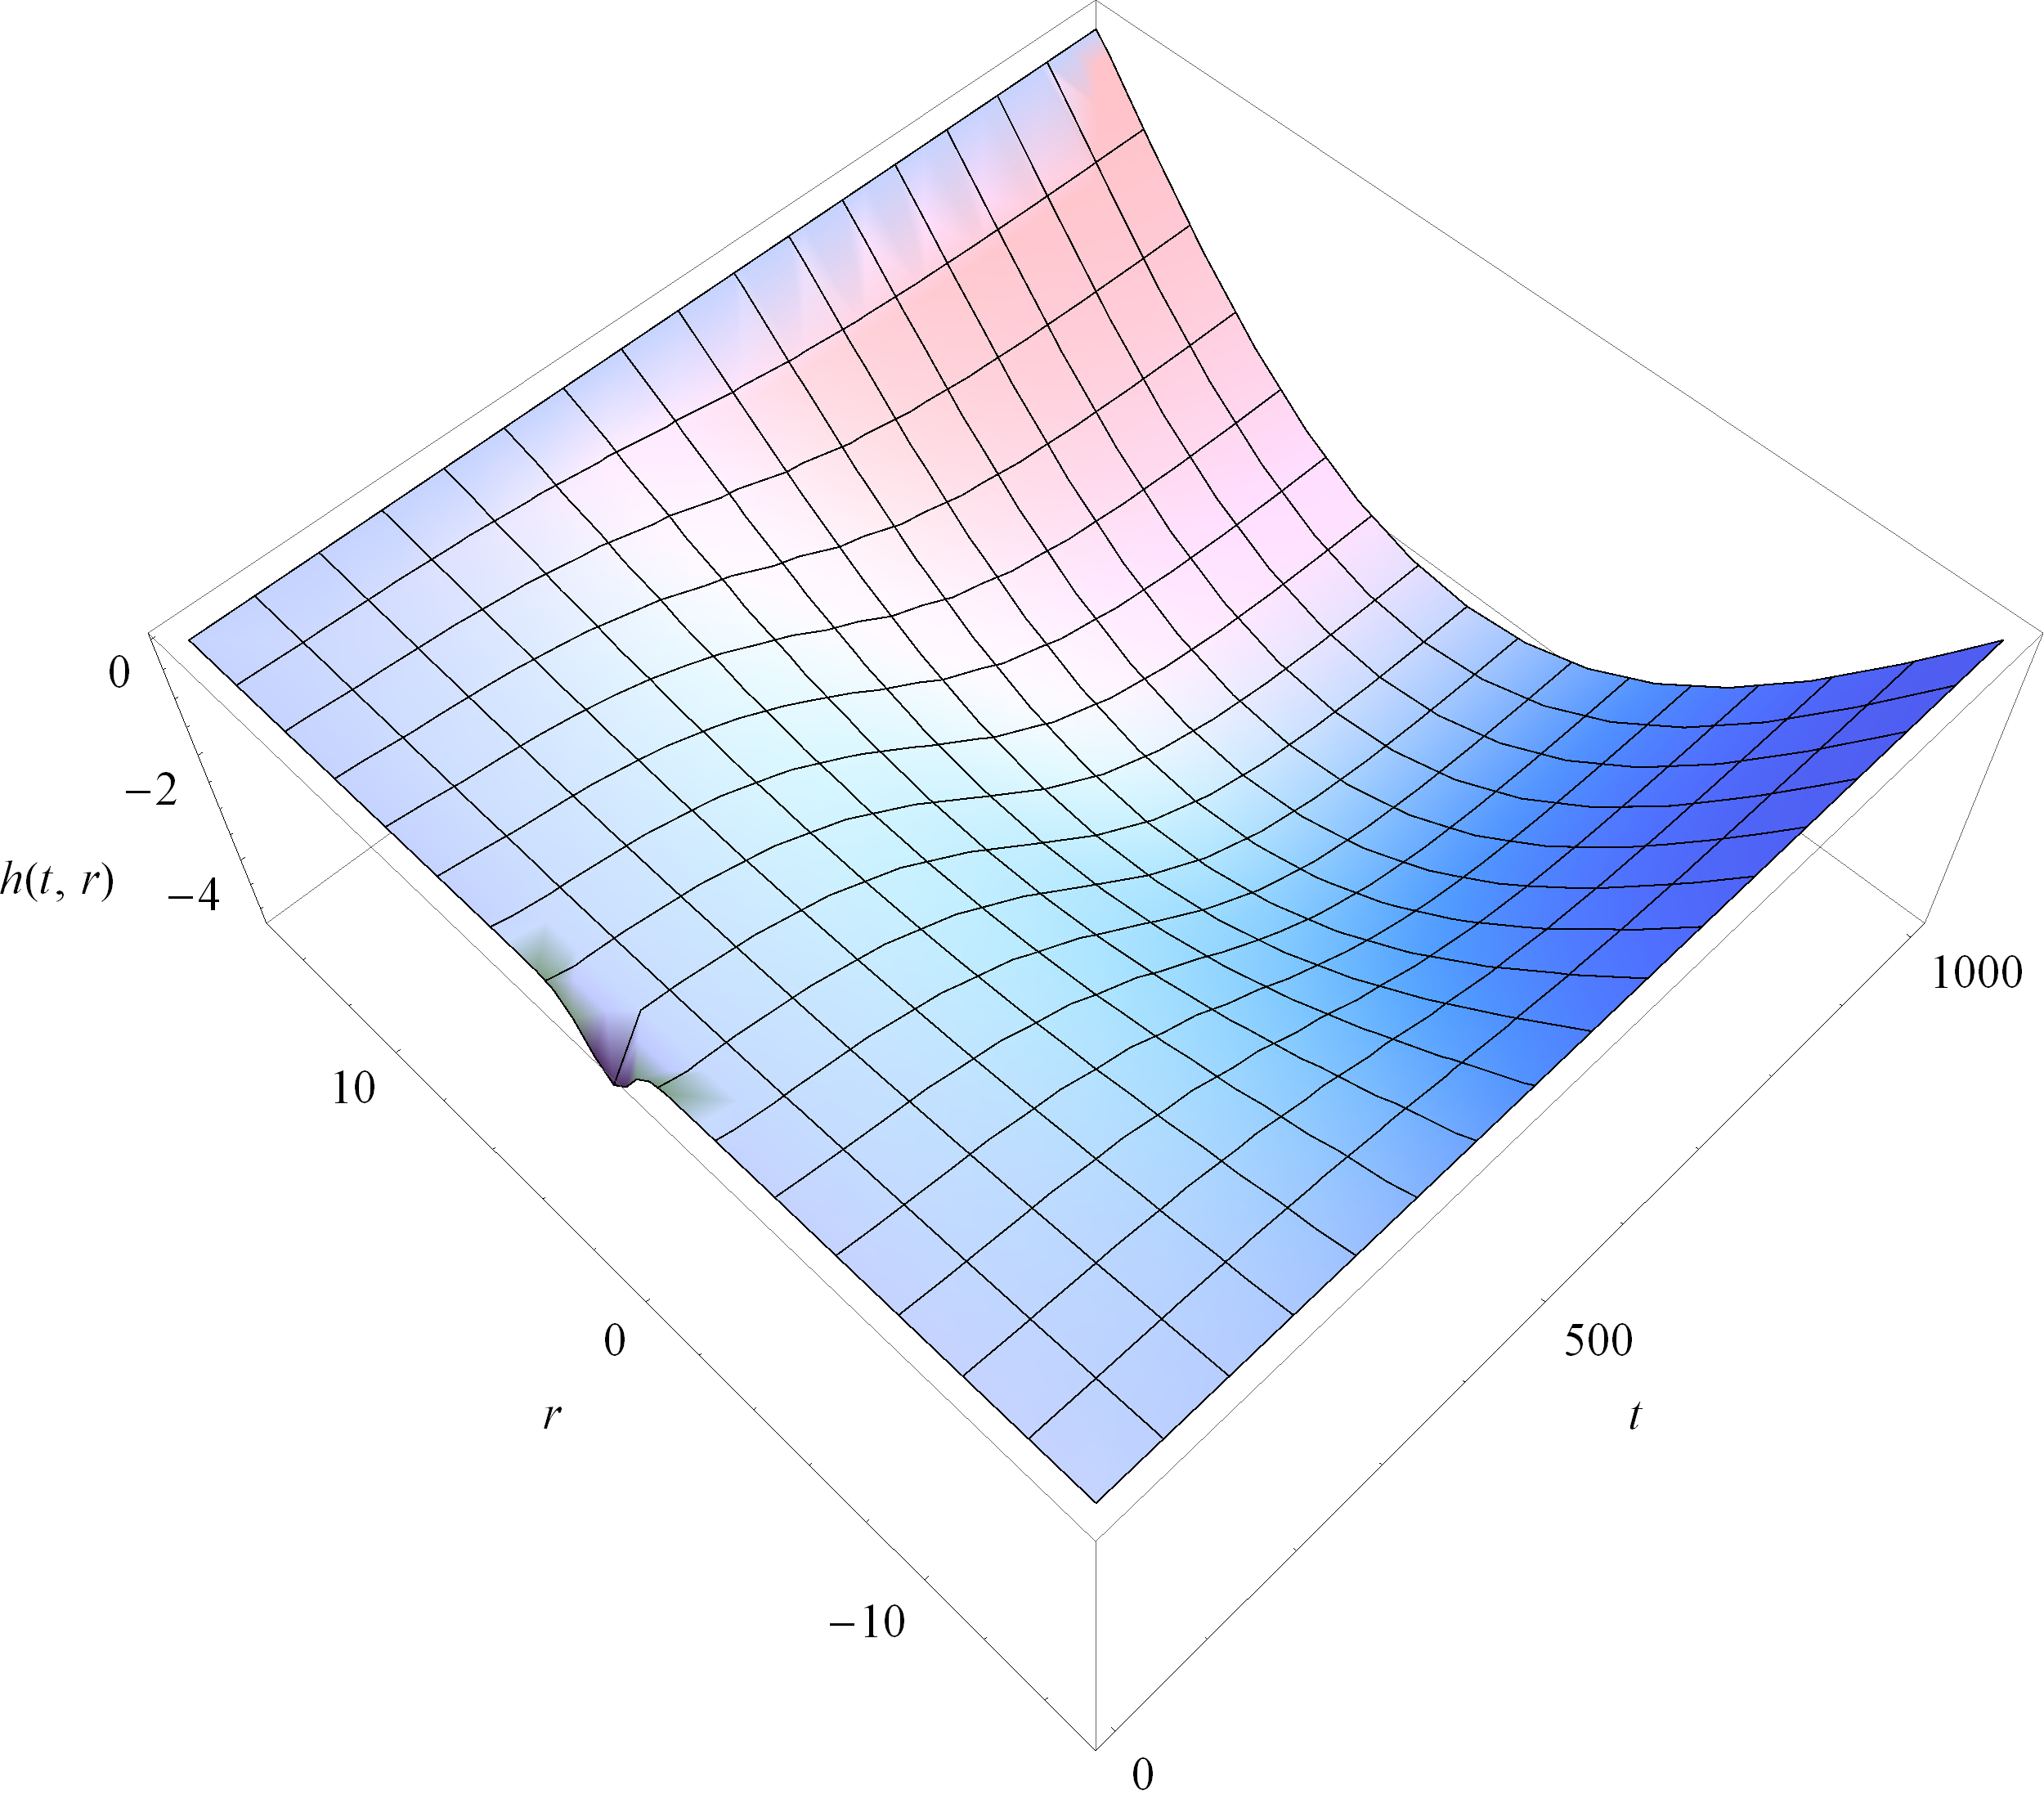
\includegraphics[width=10cm]{slike/difuzija-logisticna-rast2}
              \end{center}
              \caption{Vzeli smo $D=1$, $a=\frac{1}{50}$, $K=-10$}
              \label{fig:difuzija-logisticna-rast}
            \end{figure}

            Vidimo, da ko se pobočje enkrat oblikuje, ne spreminja več oblike, ampak potuje kot valovna fronta navzven. Pokažemo lahko, da je dolžina vala odvisna od difuzijske konstante $D$ in faktorja rasti $a$, ter da velja: 

           \[ \lambda \sim \sqrt{D/a} \]

          Iz te zveze lahko pokažemo tudi, da je hitrost takega vala $v = 2 \sqrt{D a}$.

          Enačba (\ref{difuzija-logisticna-rast}) se uporablja za opis zaželjenih genov v populaciji, širjenje populacije v neposeljenem teritoriju, itn.
          Difuzivna logistična rast se zdi pri primerno izbranem faktorju $K$ zanimiv model za dinamiko vrtač.


          \subsection{Omejena eksponentna rast}

          Če izberemo $F(h) = a \cdot (K - h)$, dobimo:

            \begin{equation}
              \frac{ \partial h(t,x) }{ \partial t} = D \Delta h(t.x) + a \cdot (K - h(t,x))
              \label{difuzija-omejena-eksponentna-rast}
            \end{equation}

            \begin{figure}[H]
              \begin{center}
                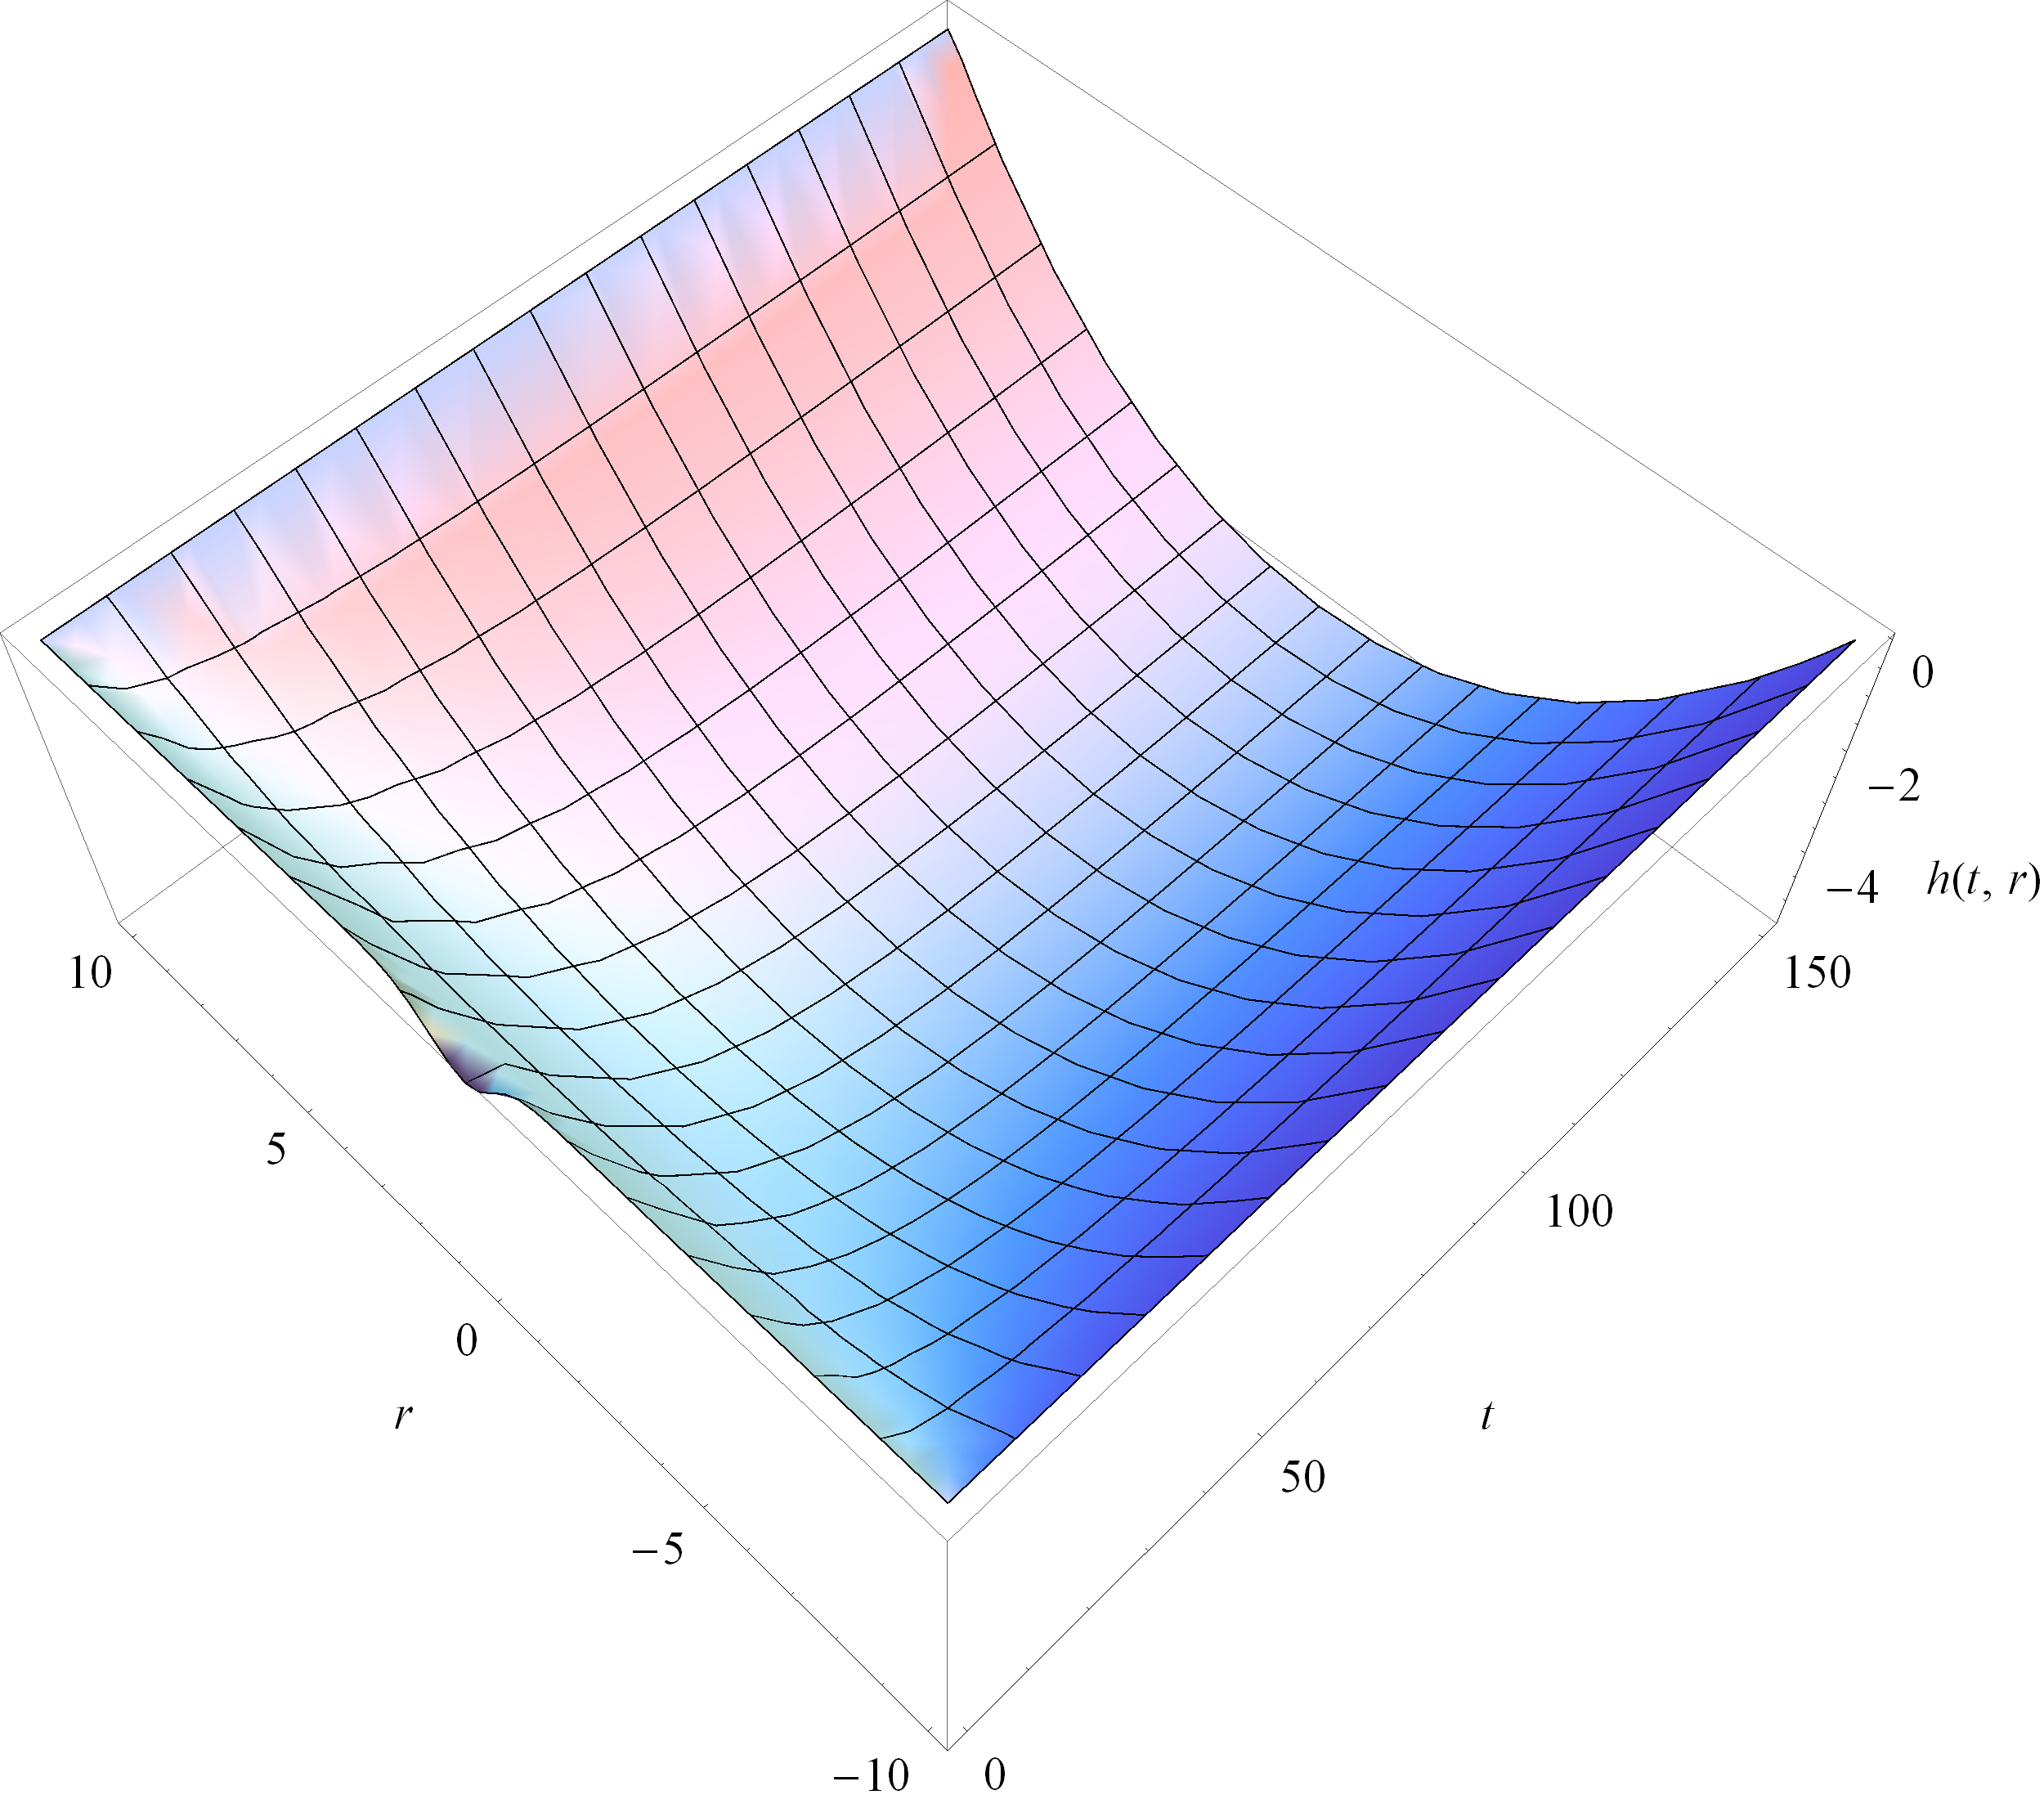
\includegraphics[width=10cm]{slike/difuzija-omejena-eksponentna-rast2}
              \end{center}
              \caption{Vzeli smo $D=1$, $a=\frac{1}{50}$, $K=-10$}
              \label{fig:difuzija-omejena-eksponentna-rast}
            \end{figure}

          Tako dobljena rast eksponentno raste do praga K, kjer se zasiti. Rast v poljubni točki je neodvisna od stanja v sosednjih. Ta model se ne zdi najbolj verjeten kandidat za dinamiko vrtač.



          \subsection{Gompertzova rast}

          Če izberemo $F(h) = - h \cdot e^{-a t}$, dobimo:

            \begin{equation}
              \frac{ \partial h(t,x) }{ \partial t} = D \Delta h(t.x) - h(t,x) \cdot e^{-a t}
              \label{difuzija-gompertzova-rast}
            \end{equation}

            \begin{figure}[H]
              \begin{center}
                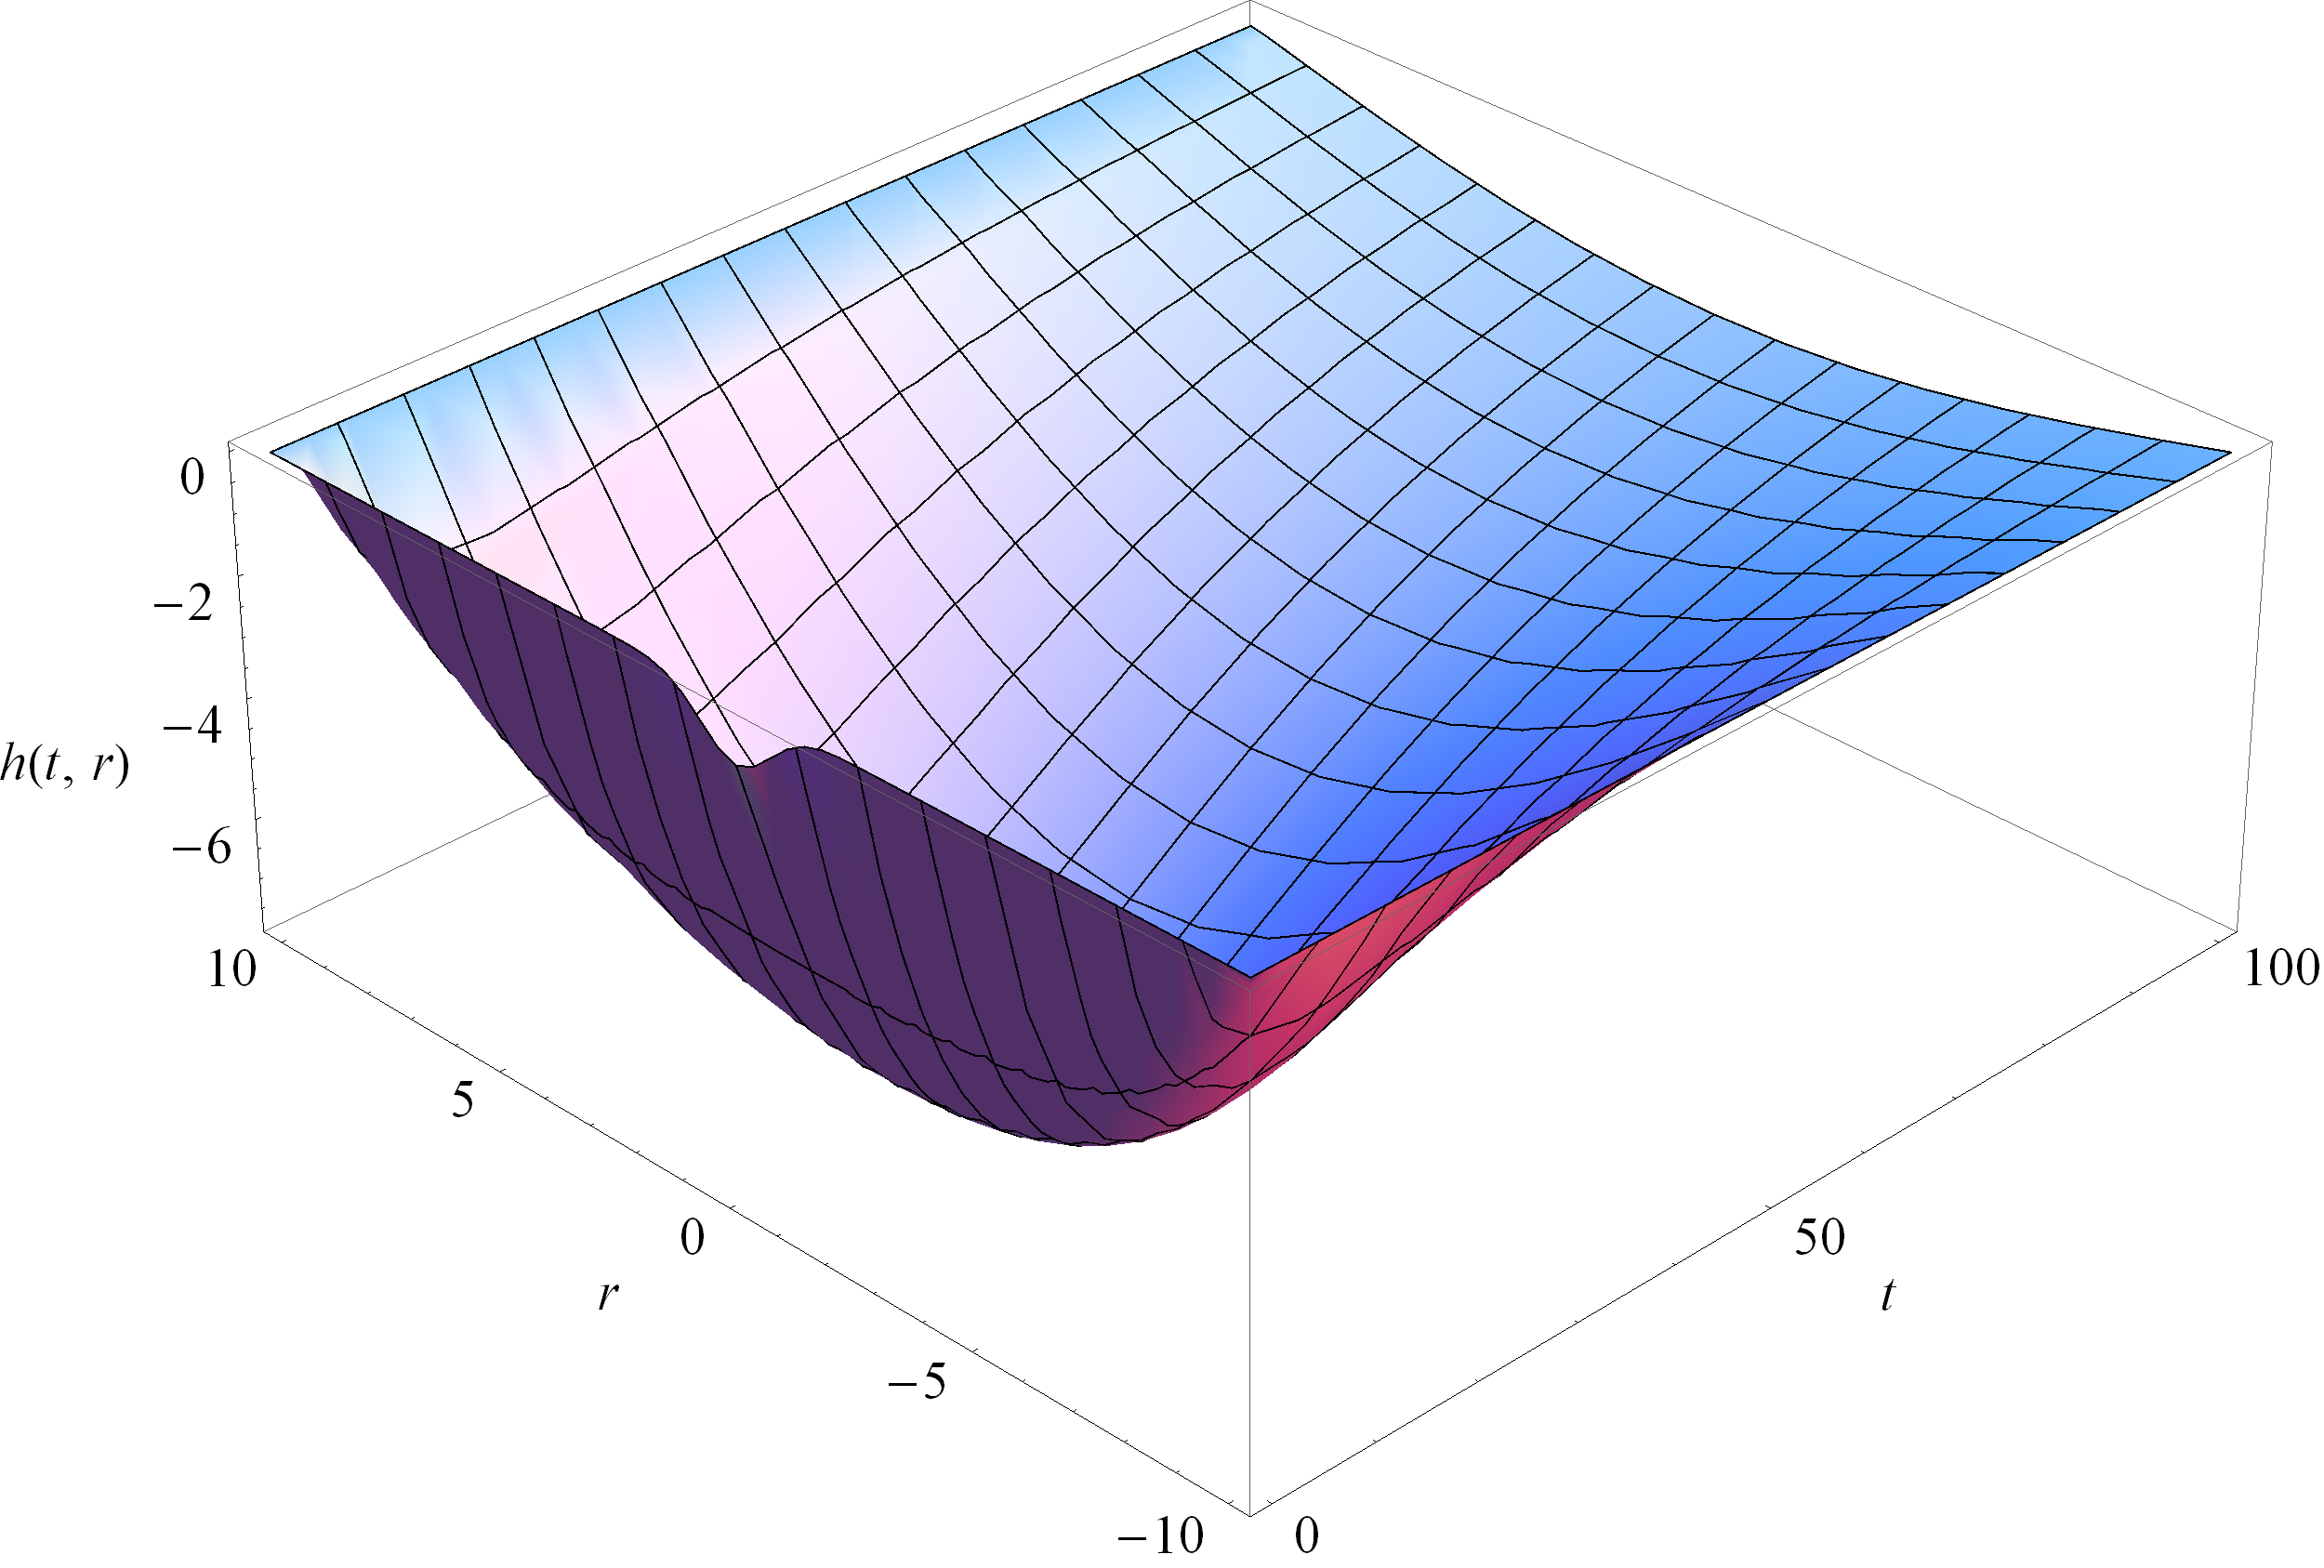
\includegraphics[width=10cm]{slike/difuzija-gompertzova-rast2}
              \end{center}
              \caption{Vzeli smo $D=1$, $a=\frac{1}{10}$}
              \label{fig:difuzija-gompertzova-rast}
            \end{figure}

            Vidimo, da rast tokrat s časom upada. Tako profil najprej zraste, nato pa se difuzijsko izravna, ko difuzija prevlada.
            Model se zdi za modeliranje vrtač neprimeren, saj nimamo jasne razlage, kaj bi povzročilo faktor rasti, ki bi nato eksponentno zamrl.


            \chapter{Zaključek}

            Izkaže se, da je zaznava in segmentacija vrtač na digitalnem modelu reliefa relativno enostavna naloga, izvedljiva na osebnem računalniku. Kodo, ki sem jo za ta postopek spisal, sem dokumentirano objavil na spletu in bo morda služila za obsežnejšo katalogizacijo vrtač.
Za nekoliko težjo nalogo se izkaže določanje idealne oblike vrtače, saj le-ta ne obstaja. Pravo vprašanje bi se moralo glasiti, kakšna je idealna oblika vrtače na izotropni podlagi po dolgem času. Vseeno sem se odločil, da za idealno vrtačo vzamem povprečje velike količine vrtač.
Precej zahtevnejša naloga je bila izbira fizikalnega modela in dinamičnega opisa vrtače zaradi omejene količine podatkov o časovni dinamiki (domnevali smo, da so vse vrtače že v ravnovesnem stanju) in nepoznavanja dejanskega procesa, ki znižuje površje.

Kardar-Parisi-Zhangova rast vmesnika nam da rezultat presenetljivo podoben kraškemu površju z vrtačami. Teoretično napovedan eksponent hrapavosti pa se relativno dobro ujema z izmerjenim na področju Menišije. Teh rezultatov ne moremo obravnavati kot dokaz, morda le vzpodbudo za nadaljni študij. V kolikor pa se model izkaže za pravilnega, pomeni spremembo v geomorfološkem kanonu, ki pravi, da se večina raztapljanja zgodi dlje od površja.

Za nepopolen model dinamike rasti vrtač predlagajmo model difuzijsko logistične rasti (\ref{fig:difuzija-logisticna-rast}), a le zato, ker se zdi najmanj napačen.

Za popolnejši študij in dober model vrtač bi verjetno potrebovali bolj poglobljene informacije o prsti, geoloških in bioloških dejavnikih, ki lahko vplivajo na časovno dinamiko terena. Zanimiva ideja bi bila z geološkim študijem najti in datirati vrtače v različnih stopnjah razvoja ter s pomočjo te informacije oblikovati dinamičen nastavek, na podlagi katerega bi potem morda bolj osvetlili dinamično enačbo.

            \nocite{*}
            \newpage
            \bibliography{bibliography}{}
            \bibliographystyle{alpha}


            \end{document}

